% This is the beamer document file of the BKU sidebar theme.
% Copyright (c) 2019/06/20 by Nguyen Van Hung <nvhung1401@gmail.com>m>.
\documentclass[
%%% options passed to the beamer
	10pt,                % font size
%	t,                   % position text on top of frame (default is c)
%	leqno,               % equation numbering on the left (default is on the right)
%	fleqn,               % equation is on the left (default is in the middle)
	aspectratio=169,     % aspect ratio (default is 4:3)
%	handout,             % disable "\pause" and "\only" mode
]{beamer}


%%%%%%%%%%%%%%%%%%%%%%%%%%%%%%%%%%%%%%%%%%%%%%%%
% Load theme
%%%%%%%%%%%%%%%%%%%%%%%%%%%%%%%%%%%%%%%%%%%%%%%%
\usetheme[
%%% options passed to the outer theme
%	left,                % right of left position of sidebar (default is right)
	width=2.25cm,        % width of the sidebar (default is 2 cm)
%	hidetitle,           % hide the (short) title in the sidebar
%	hideauthor,          % hide the (short) author in the sidebar
	hideothersubsections,% hide all subsections but the subsections in the current section
%	hideallsubsections,  % hide all subsections
%	hideinstitute,       % hide the (short) institute in the bottom of the sidebar
%	shownavsym,          % show the navigation symbols
%%% options passed to the inner theme
%	transparent,         % install animation
%%% options passed to the color theme
	lightheaderbg,       % use a light header background
]{BKUsidebar}

% end of load theme

%%%%%%%%%%%%%%%%%%%%%%%%%%%%%%%%%%%%%%%%%%%%%%%%
% Load package and definitions
%%%%%%%%%%%%%%%%%%%%%%%%%%%%%%%%%%%%%%%%%%%%%%%%

\uselanguage{vietnamese}                        % "english" or "vietnamese"
\usepackage{multicol}                           % provides multicolumn environment
\usepackage{graphicx}                           % provides commands about graphic
\usepackage{ragged2e}                           % provides justify command
\usepackage{verbatim}                           % provides verbarim environment
\usepackage{xcolor}                             % provides commands about color
\usepackage{subcaption}							% provides environment for subfigure
\usepackage{booktabs}							% provides more rules in talble
\usepackage{multirow}							% provides multirow in table
\usepackage{pgfplots}							% plot fuction in tikz
\usepackage{pgfgantt}
\usepackage{makecell}
\newcommand\Dganttbar[4]{
	\ganttbar{#1}{#3}{#4}\ganttbar[inline,bar label font=\footnotesize]{#2}{#3}{#4}
}

\definecolor{commentcolor}{RGB}{0,128,58}       % green
\definecolor{keywordcolor}{RGB}{55,0,255}       % blue
\definecolor{stringcolor}{RGB}{167,21,62}       % dark red
\definecolor{backgroundcolor}{RGB}{30,30,30}    % dark gray
\lstset
{
	language=C++,                               % language programming
	basicstyle=\ttfamily,                       % type for basic
	keywordstyle=\bfseries\color{keywordcolor}, % type for keywords
	identifierstyle=\color{black},              % type for identifier
	stringstyle=\color{stringcolor},            % type for string
	commentstyle=\color{commentcolor},          % type for comment
	emph={iostream},                            % first list of another word
	emphstyle=\color{stringcolor},              % type for first list of another word
%	emph={[2]word3},                            % second list of another word
%	emphstyle=[2]\color{red},                   % type for second list of another word
	tabsize=2,                                  % width of tab
%	showtabs=true,                              % enable character tab
%	tab=\rightarrowfill,                        % character tab
%	showspaces=true,                            % enable character spaces in all code
	showstringspaces=true,                      % enable character spaces in string
	breaklines=true,                            % enable breaklines mode
	escapechar=\@,                              % character to back to LaTeX mode
	numbers=left,                               % lines numbering on left
	numberstyle=\normalsize,                    % stype for lines number
%	firstnumber=100,                            % first number counting for lines number
	stepnumber=1,                               % step lines numbering
	numbersep=5pt,                              % space between lines number and code
%	frame=leftline,                             % insert line for lines numbering
%	frame=single,                               % insert box with single line
%	framerule=1pt,                              % width of line of box
	xleftmargin=5mm,                            % left margin
%	xrightmargin=1cm,                           % right margin
%	backgroundcolor=\color{backgroundcolor},    % white background
	captionpos=b,                               % position of caption
}

\newcommand\footnotesource[1]{					% footnote for data source
	\vspace{-10mm}\let\thefootnote\relax\footnote{\hspace{-3mm}\tiny Nguồn:~#1}
}

\usepackage{multirow, booktabs}

\usepackage[
    backend=biber,
    style=alphabetic,
    sorting=ynt
    ]{biblatex}
% \addbibresource{ref.bib}

% end of load package and definitions


%%%%%%%%%%%%%%%%%%%%%%%%%%%%%%%%%%%%%%%%%%%%%%%%
% Information on title page
%%%%%%%%%%%%%%%%%%%%%%%%%%%%%%%%%%%%%%%%%%%%%%%%
\lecture
	{}
	{2020/09/21}
\title
	[Hệ thống làm nhãn cho ảnh chụp cắt lớp vi tính (CT) với sự trợ giúp của Trí tuệ nhân tạo]% optional, use only with long paper titles
	{\scalebox{.84}[1]{HỆ THỐNG LÀM NHÃN CHO ẢNH CHỤP CẮT  }\\\scalebox{.84}[1]{LỚP VI TÍNH VỚI SỰ TRỢ GIÚP CỦA TRÍ TUỆ}\\\scalebox{.84}[1]{NHÂN TẠO}}
\subtitle
	{Luận văn tốt nghiệp (CO4313)}% could also be a subject name
\subject
	{TP. Hồ Chí Minh}% could also be address
%\reference
%	{reference}
\institute
	[Khoa KH - KT Máy tính\\Đại học Bách Khoa]% optional - use only with long paper institute
	{Khoa Khoa học - Kỹ thuật Máy tính\\Đại học Bách Khoa - Đại học quốc gia TP.HCM}
\instructor
	{GVHD: \\ \\GVPB: }
	{ TS. Lê Thành Sách\\ TS. Nguyễn Hồ Mẫn Rạng\\ TS. Trần Tuấn Anh}% use "\\" between instructors with lots of instructors
\student
	[SVTH: ]% must be inserted if instructor inserted
	{Cao Thanh Tùng\\ Nguyễn Thanh Tuấn \\ Phan Ngọc Thịnh}% use "\\" between students with lots of students
	{1613989\\ 1613907 \\ 1613361}% Similar to students

% end of information on title page

%%%%%%%%%%%%%%%%%%%%%%%%%%%%%%%%%%%%%%%%%%%%%%%%
% Main content
%%%%%%%%%%%%%%%%%%%%%%%%%%%%%%%%%%%%%%%%%%%%%%%%

\begin{document}

%-The-title-page--------------------------------
\begin{frame}[noframenumbering]
	\titlepage
\end{frame}

%-TOC-------------------------------------------
\section*{Mục lục}
	\begin{frame}{Mục lục}
		\hfill
		\parbox[c]{.98\textwidth}{
			\vspace{-3mm}
			\tableofcontents[hideallsubsections]% the hideallsubsections option removes subsection/subsubsection in TOC
		}
	\end{frame}

%-Contents--------------------------------------
\section{Tổng quan}

\subsection{Giới thiệu đề tài}
	\begin{frame}{Tổng quan}{Giới thiệu đề tài}
	    \begin{block}{Động lực thực hiện}
			\begin{enumerate}
				\item Tỉ lệ tử vong do ung thư gan tại Việt Nam cao.
				\item Ứng dụng trí tuệ nhân tạo vào lĩnh vực y học trở nên phổ biến.
			\end{enumerate}
		\end{block}
		\vspace{-0.2cm}
		\begin{figure}[h!]
			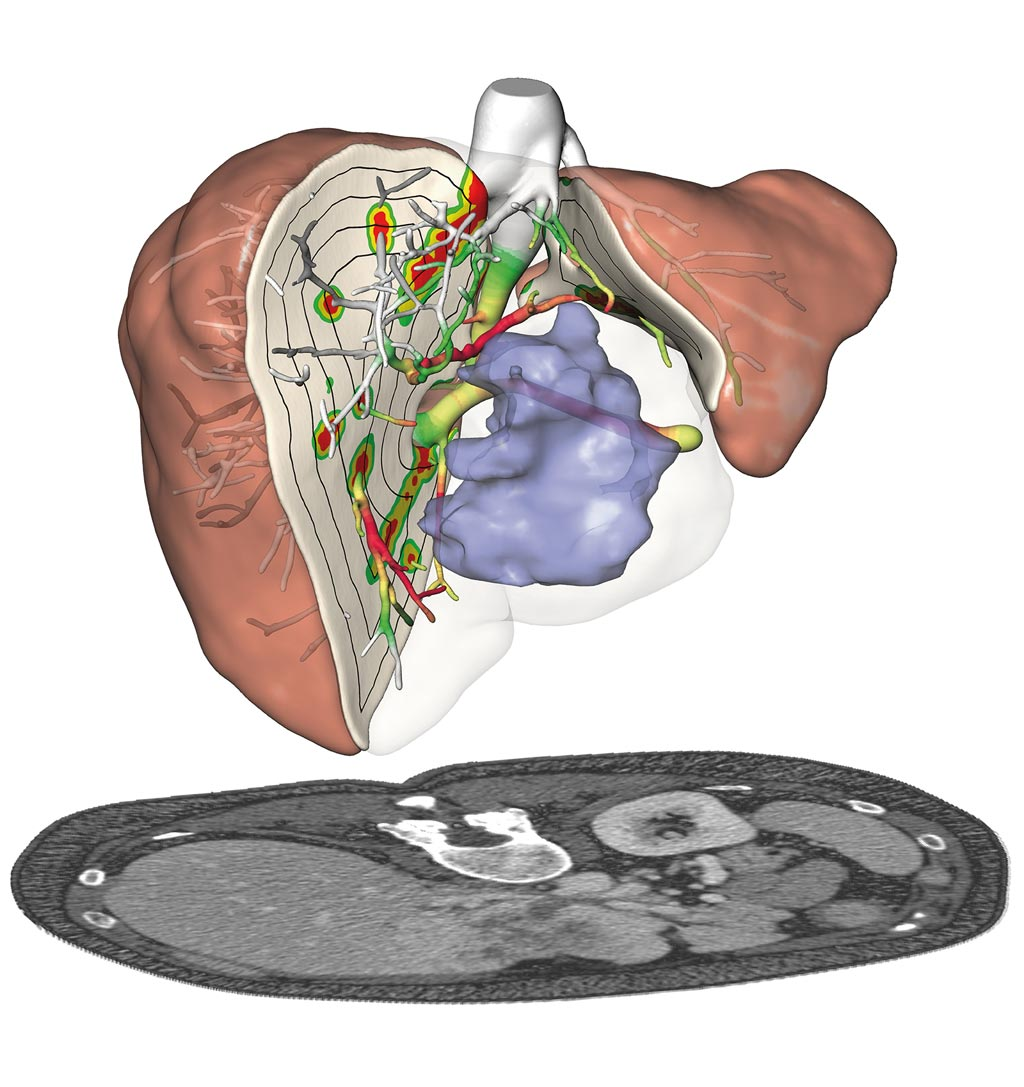
\includegraphics[scale=0.1]{Presentation_template/figures/medical_CT.jpg}
			\caption{Cơ quan gan trong cơ thể người.}
		\end{figure}
		\footnotesource{ \url{https://globetechcdn.com/medicalimaging/images/stories/articles/article_images/2018-06-07/SDD-476.jpg}}
	\end{frame}

\subsection[Mục tiêu và phạm vi]{Mục tiêu và phạm vi đề tài}
	\begin{frame}{Tổng quan}{Mục tiêu và phạm vi đề tài}
	    \vspace{2mm}
		\begin{figure}[h!]
			\begin{subfigure}[b]{0.47\textwidth}
    			\centering	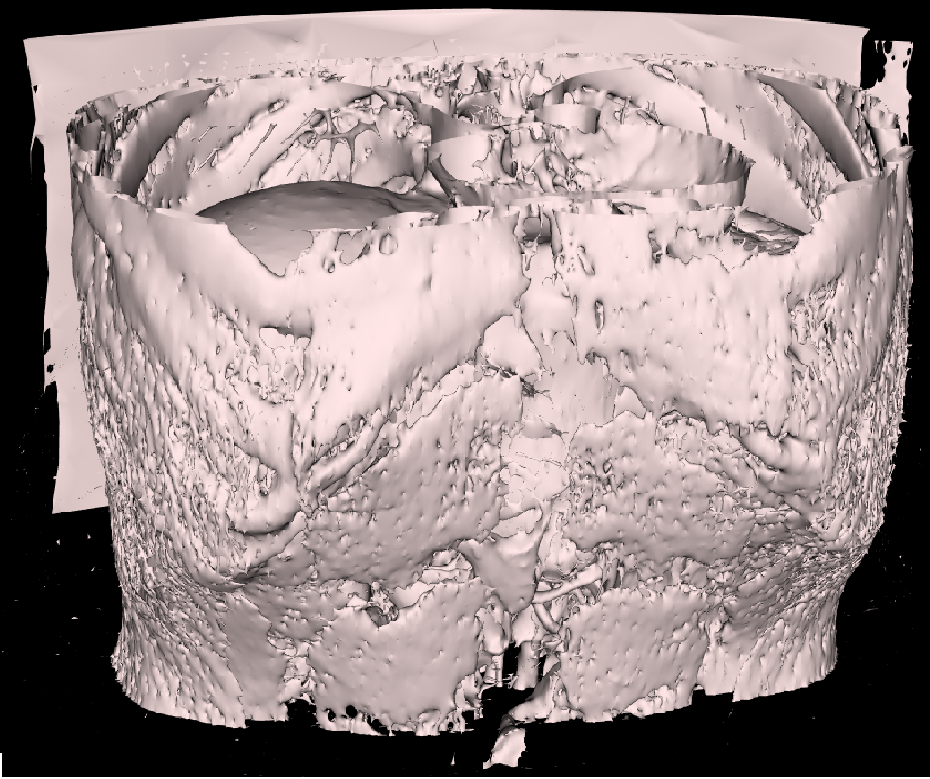
\includegraphics[scale=0.19]{Presentation_template/figures/volume-3d.png}
    			\vspace{-1mm}
    			\caption{Trực quan ảnh CT ban đầu dưới dạng 3D.}
			\end{subfigure}
			\begin{subfigure}[b]{0.5\textwidth}
    			\centering	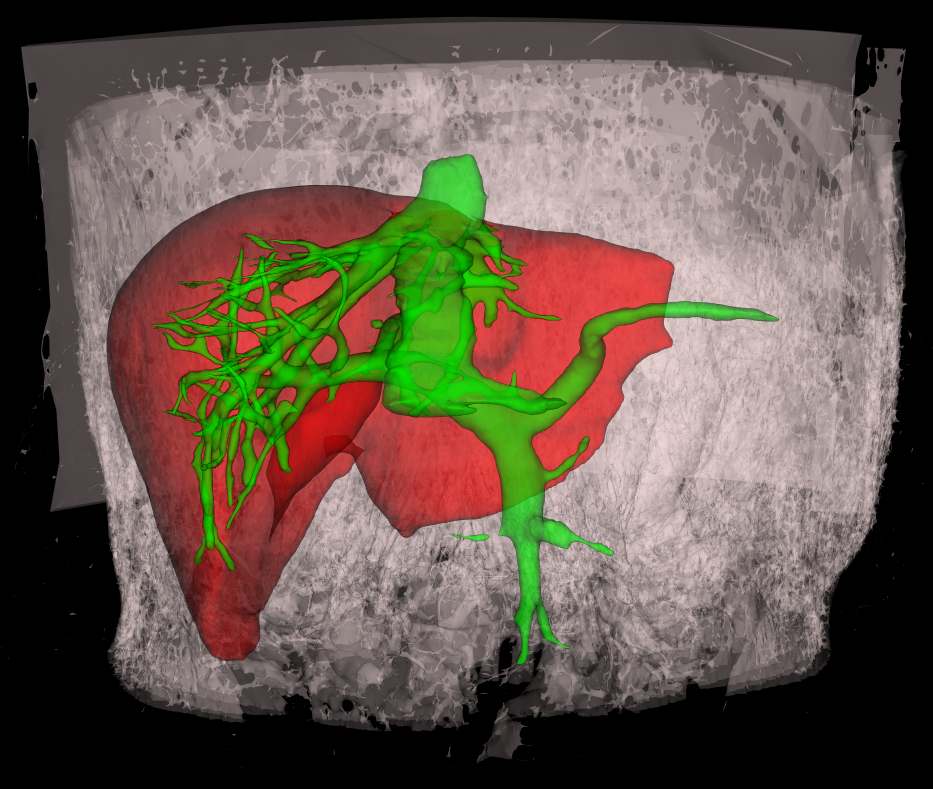
\includegraphics[height=.35\textheight]{Presentation_template/figures/liver-vessel-3d.png}
    			\vspace{-1mm}
    			\caption{Kết quả sau khi phân đoạn gan và mạch máu.}
			\end{subfigure}
		\end{figure}
		\vspace{-3mm}
		\begin{block}{Mục tiêu và phạm vi đề tài}
			\begin{enumerate}
				\item Phân đoạn gan.
				\item Phân đoạn mạch máu của gan.
				\item Kế thừa và phát triển hệ thống làm nhãn ảnh y khoa.
			\end{enumerate}
		\end{block}
	\end{frame}
	
\subsection[Thách thức]{Thách thức của đề tài}
	\begin{frame}{Tổng quan}{Những thách thức}
		\vspace{1mm}
		\begin{figure}[h!]
			\begin{subfigure}[b]{0.45\textwidth}
				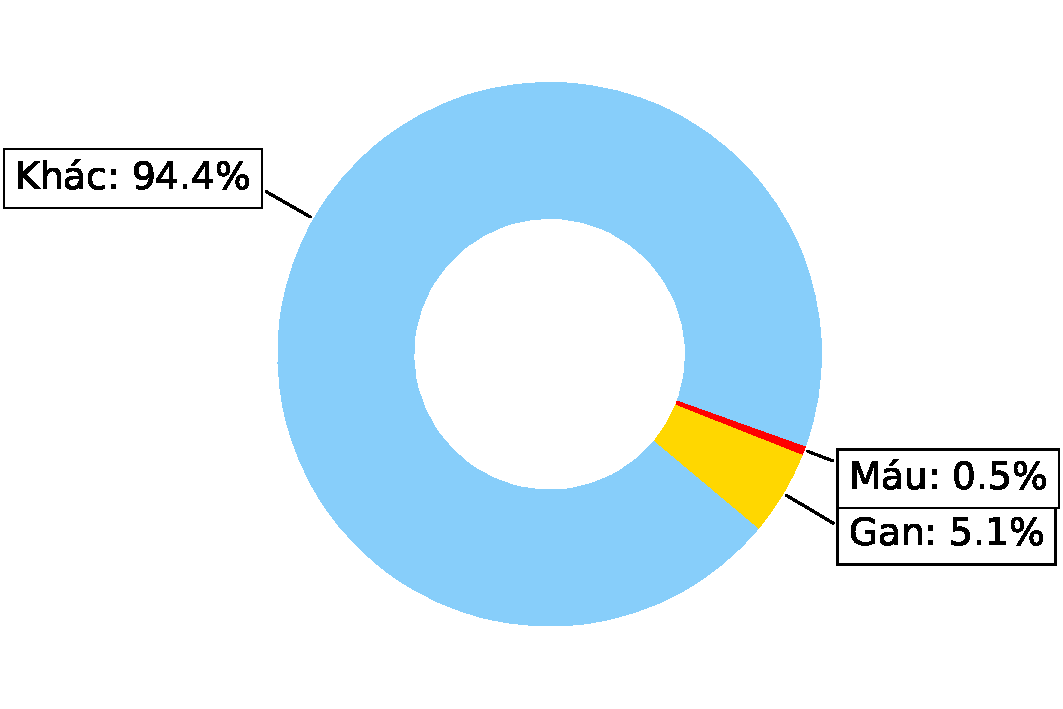
\includegraphics[height=.35\textheight]{Presentation_template/figures/liver-vessel-bg-ratio.pdf}
				\caption{Tỉ lệ gan, mạch máu trong ảnh CT.}
			\end{subfigure}
			\begin{subfigure}[b]{0.45\textwidth}
			\centering
				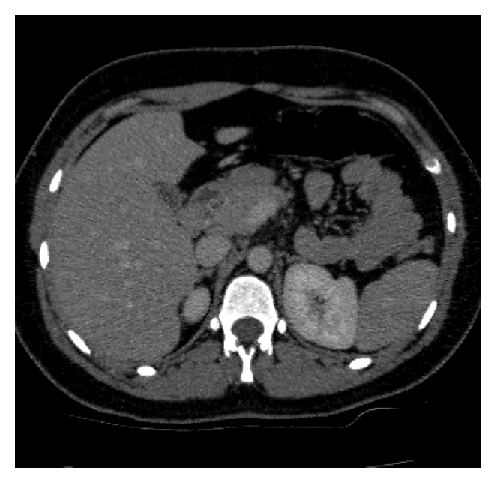
\includegraphics[height=.35\textheight]{Presentation_template/figures/ct-low-constrast.pdf}
				\caption{Một lát cắt ảnh CT.}
			\end{subfigure}
		\end{figure}
		\vspace{-3mm}
		\begin{block}{Những thách thức của đề tài}
			\begin{enumerate}
				\item Hạn chế về số lượng dữ liệu.
				\item Mất cân bằng dữ liệu.
				\item Độ tương phản thấp.
				\item Chi phí tính toán cao.
			\end{enumerate}
		\end{block}
	\end{frame}

\section{Kiến thức nền tảng}
\subsection{Mô hình mạng U-Net}
	\begin{frame}{Mô hình mạng U-Net}
		\begin{figure}
			\centering
			\vspace{-0.55cm}
			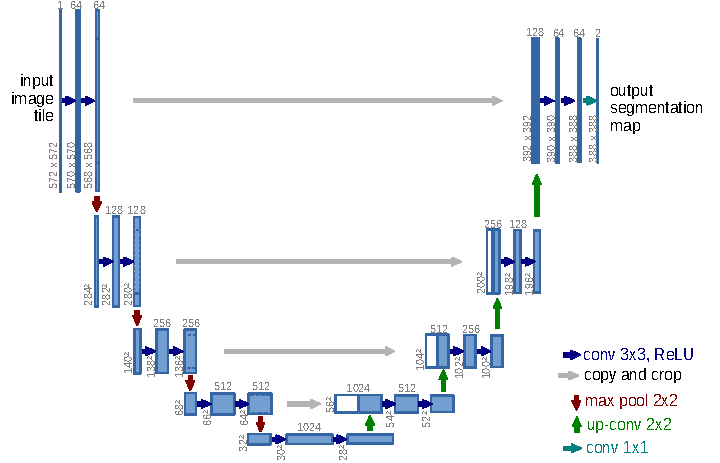
\includegraphics[scale=0.9]{figures/model_unet.pdf}
		\end{figure}
		\footnotesource{O. Ronneberger, P. Fischer, and T. Brox, ``U-net: Convolutional networks for biomedical image segmentation,'' in International Conference on Medical image computing and computer-assisted intervention, Springer, 2015, pp. 234–241.} 
	\end{frame}
	
\subsection{Mô hình mạng $U^2$Net}
	\begin{frame}{Mô hình mạng $U^2$Net}
	\vspace{-0.7cm}
	\begin{figure}
		\centering
		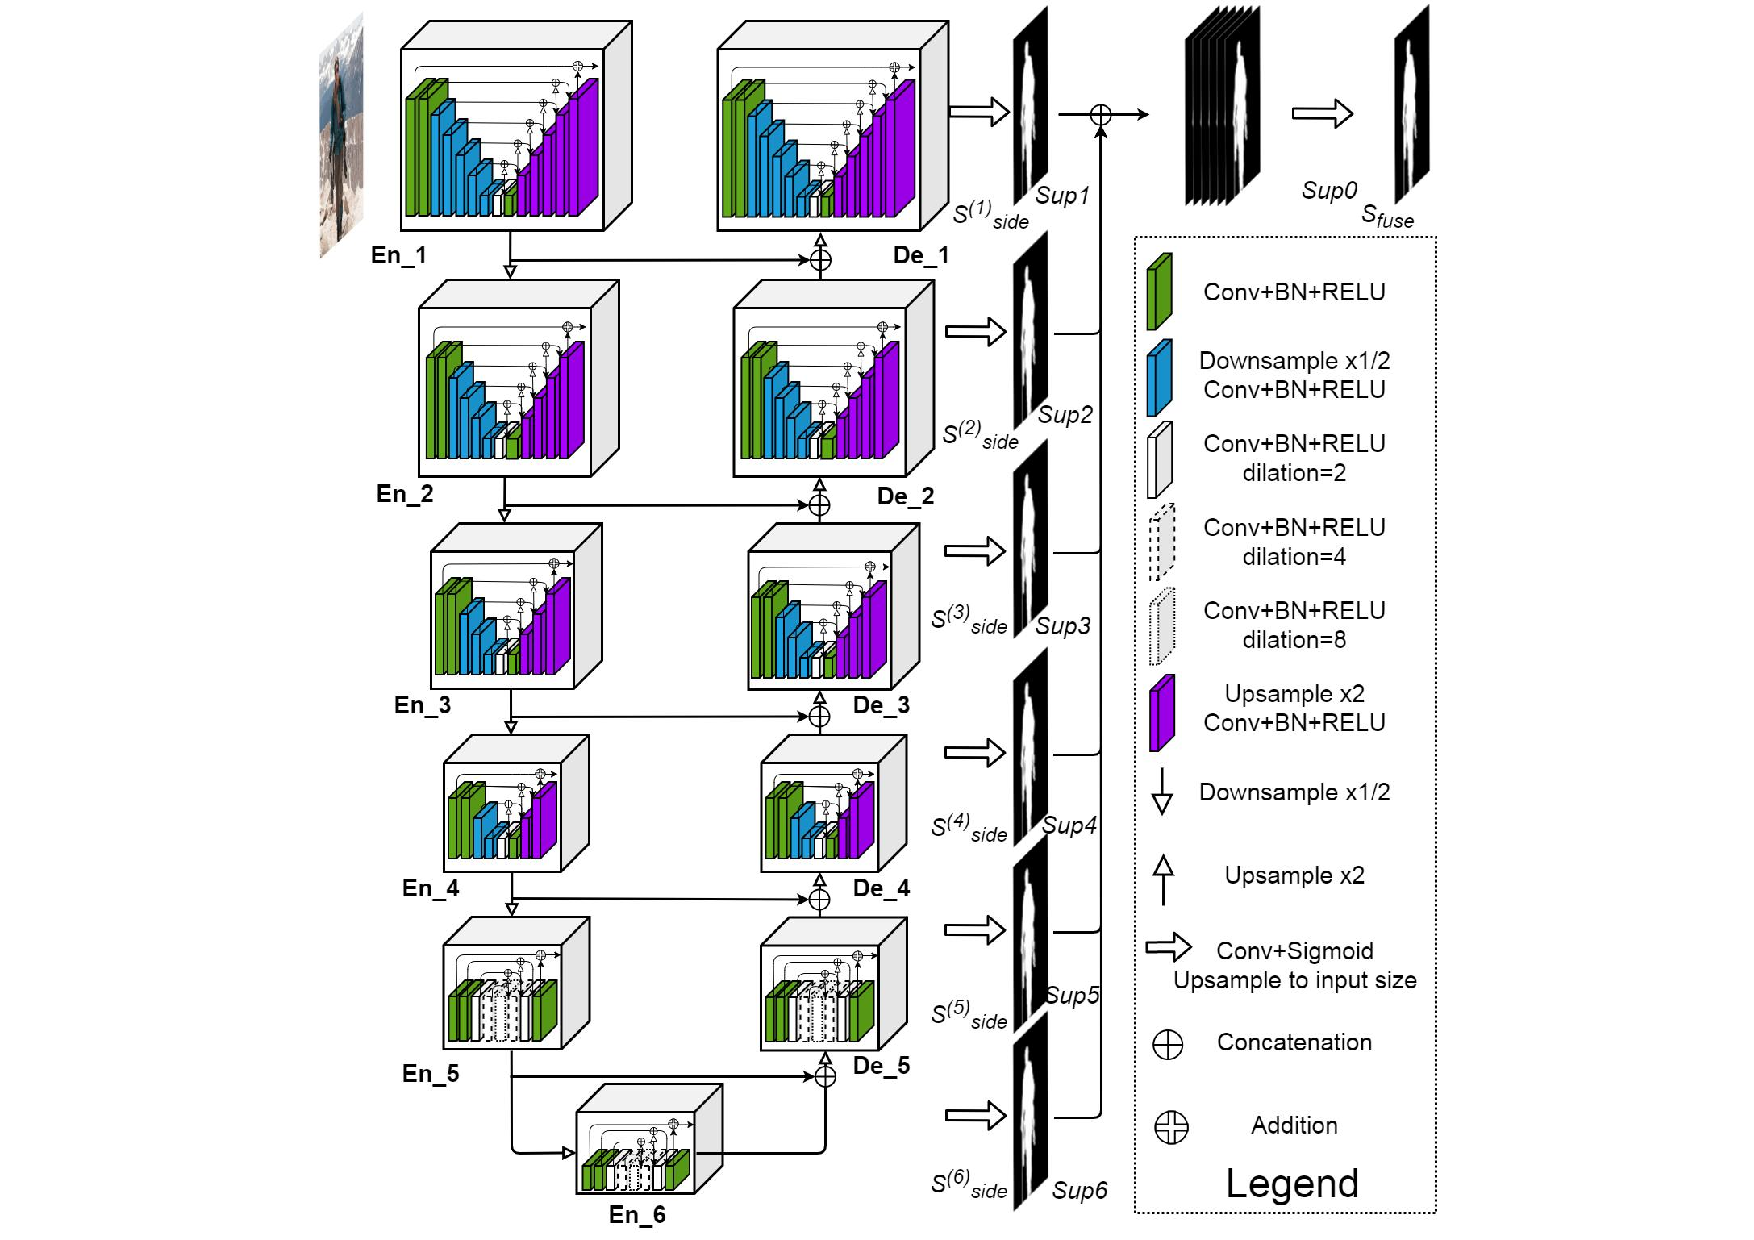
\includegraphics[scale=0.35]{figures/u2net_arch.pdf}
	\end{figure}
	\footnotesource{Qin, Xuebin, Zhang, Zichen, Huang, Chenyang, Dehghan, Masood, Zaiane, Osmar R., Jagersand, Martin ``U2-Net: Going deeper with nested U-structure for salient object detection'', 2020} 
	\end{frame}
	
\subsection{Mô hình mạng CNN3D}
	\begin{frame}{Mô hình CNN3D với giám sát sâu}
	\vspace{2mm}
		\begin{figure}
			\centering
			\vspace{-0.8cm}
			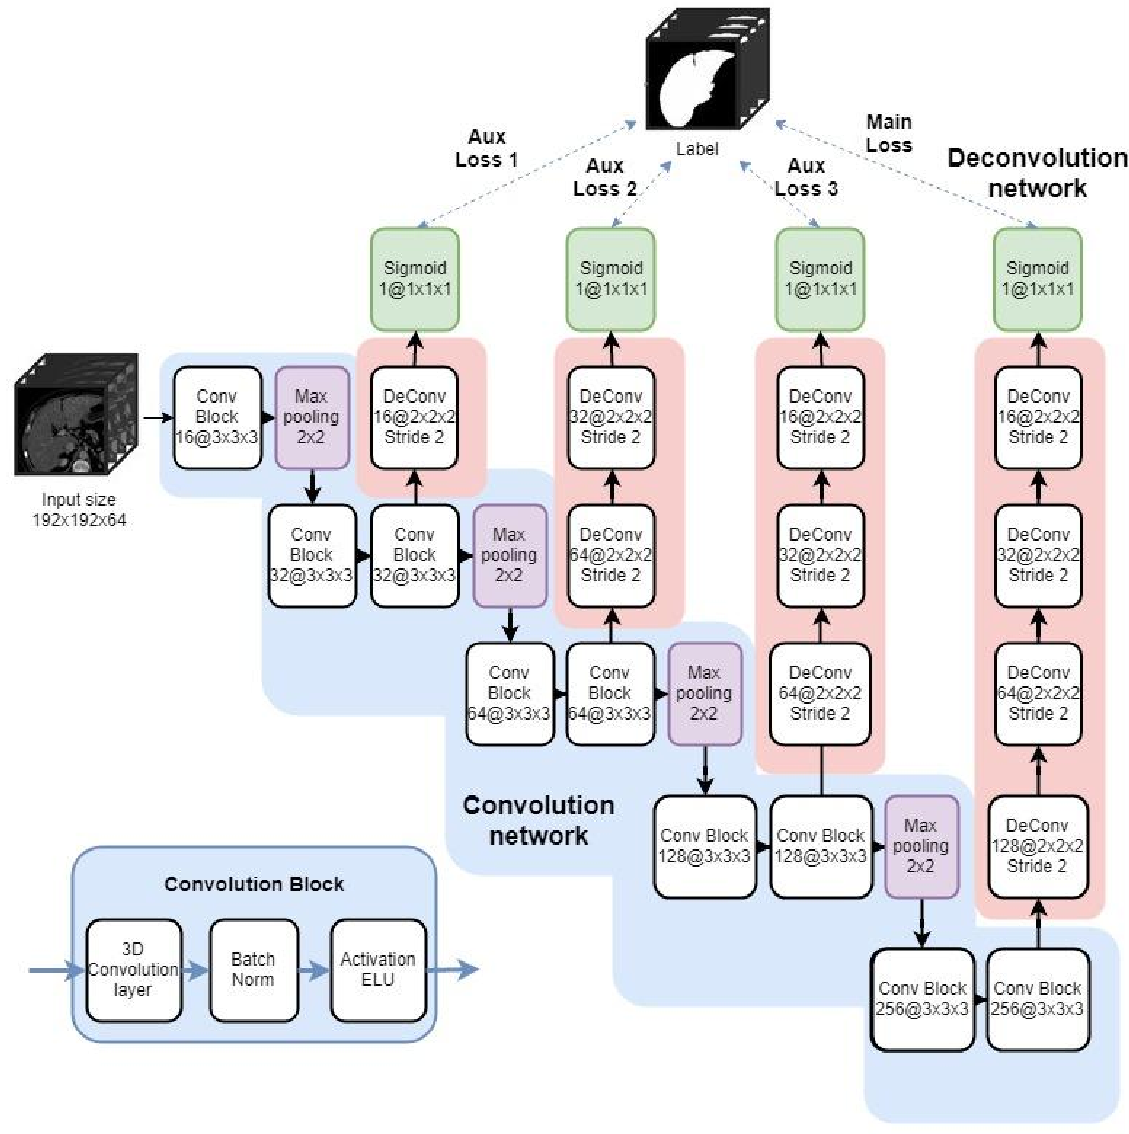
\includegraphics[scale=0.4]{Presentation_template/figures/cnn3d1.pdf}
        \end{figure}
		\footnotesource{N.Q.Hà, M.D.Tú và T.Q.Pháp,``Xây dựng mô hình gan từ ảnh chụp cắt lớp vi tính'', LVTN, 2019} 
	\end{frame}



\section{Phương án đề xuất}
\subsection{Kiến trúc mô hình}
	\begin{frame}{Kiến trúc mô hình tổng quát}
		\vspace{-0.3cm}
		\begin{figure}[h!]
			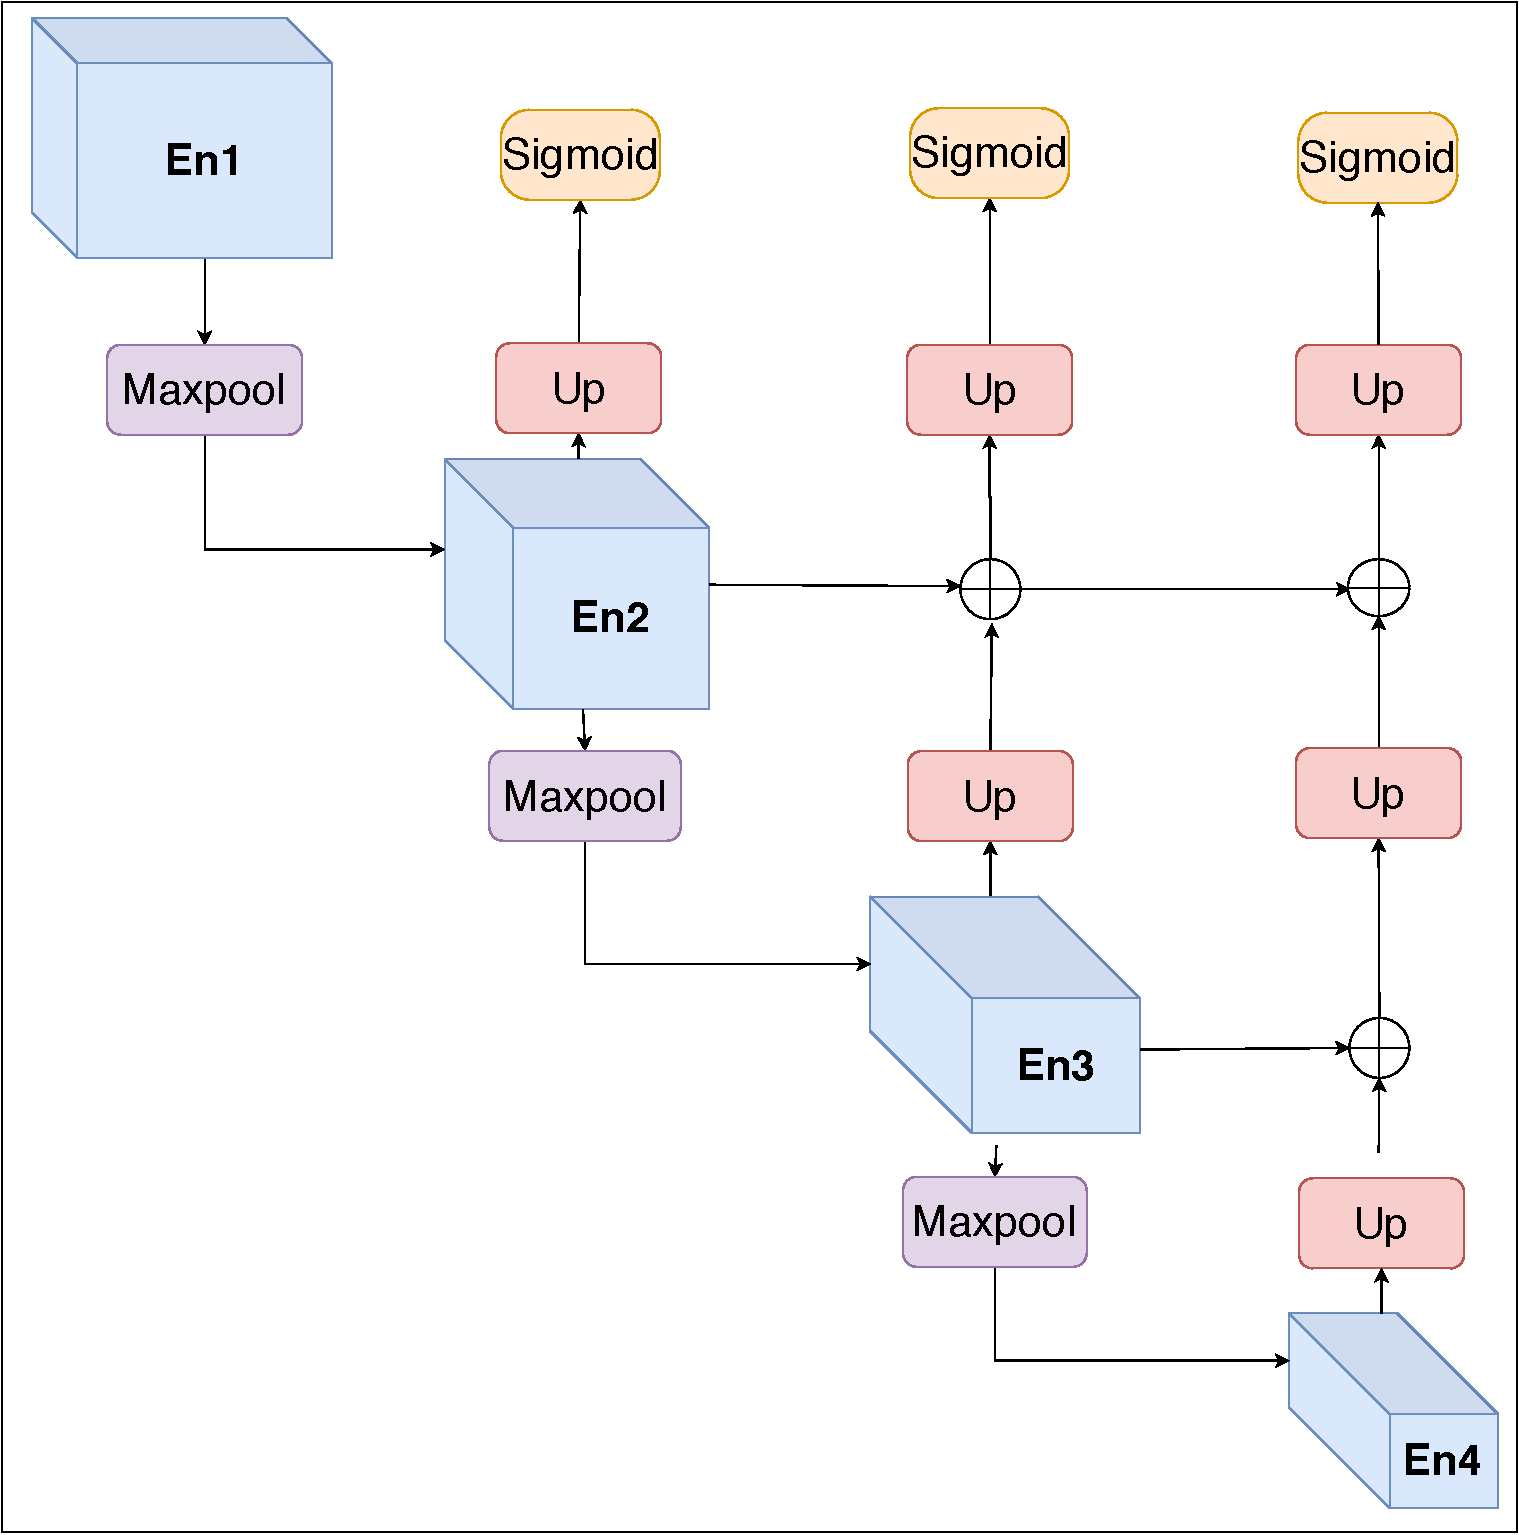
\includegraphics[scale=0.3]{figures/arch/u2net3d-abstract.pdf}
		\end{figure}
	\end{frame}
	
\subsection{Các khối tính toán}
    \begin{frame}{Các khối tính toán}
        \begin{figure}[h!]
			\begin{subfigure}[b]{0.5\textwidth}
			    \centering	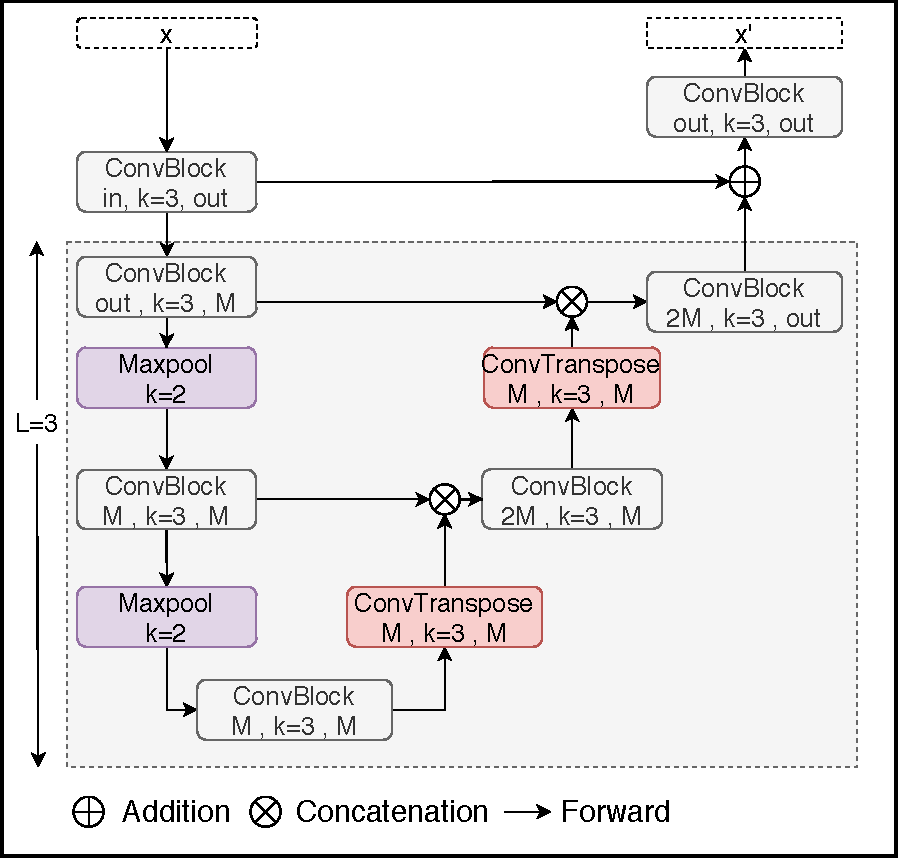
\includegraphics[scale=0.45]{figures/arch/RSU_L3.pdf}
				\caption{Residual U-Block RSU-L(In, M, Out)}
			\end{subfigure}
			\begin{subfigure}[b]{0.4\textwidth}
			    \centering	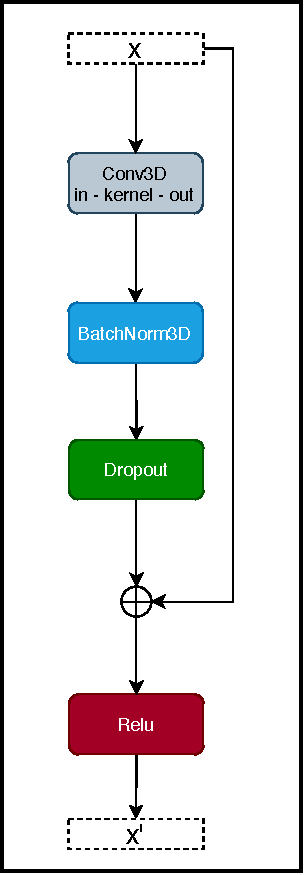
\includegraphics[scale=0.45]{figures/arch/convblock.pdf}
				\caption{ConvBlock(In, M, Out)}
			\end{subfigure}
			\vspace{-3mm}
		\end{figure}
    \end{frame}%------------------------------
    
	\begin{frame}{Kiến trúc mô hình chi tiết}
		\vspace{-0.3cm}
		\begin{figure}[h!]
			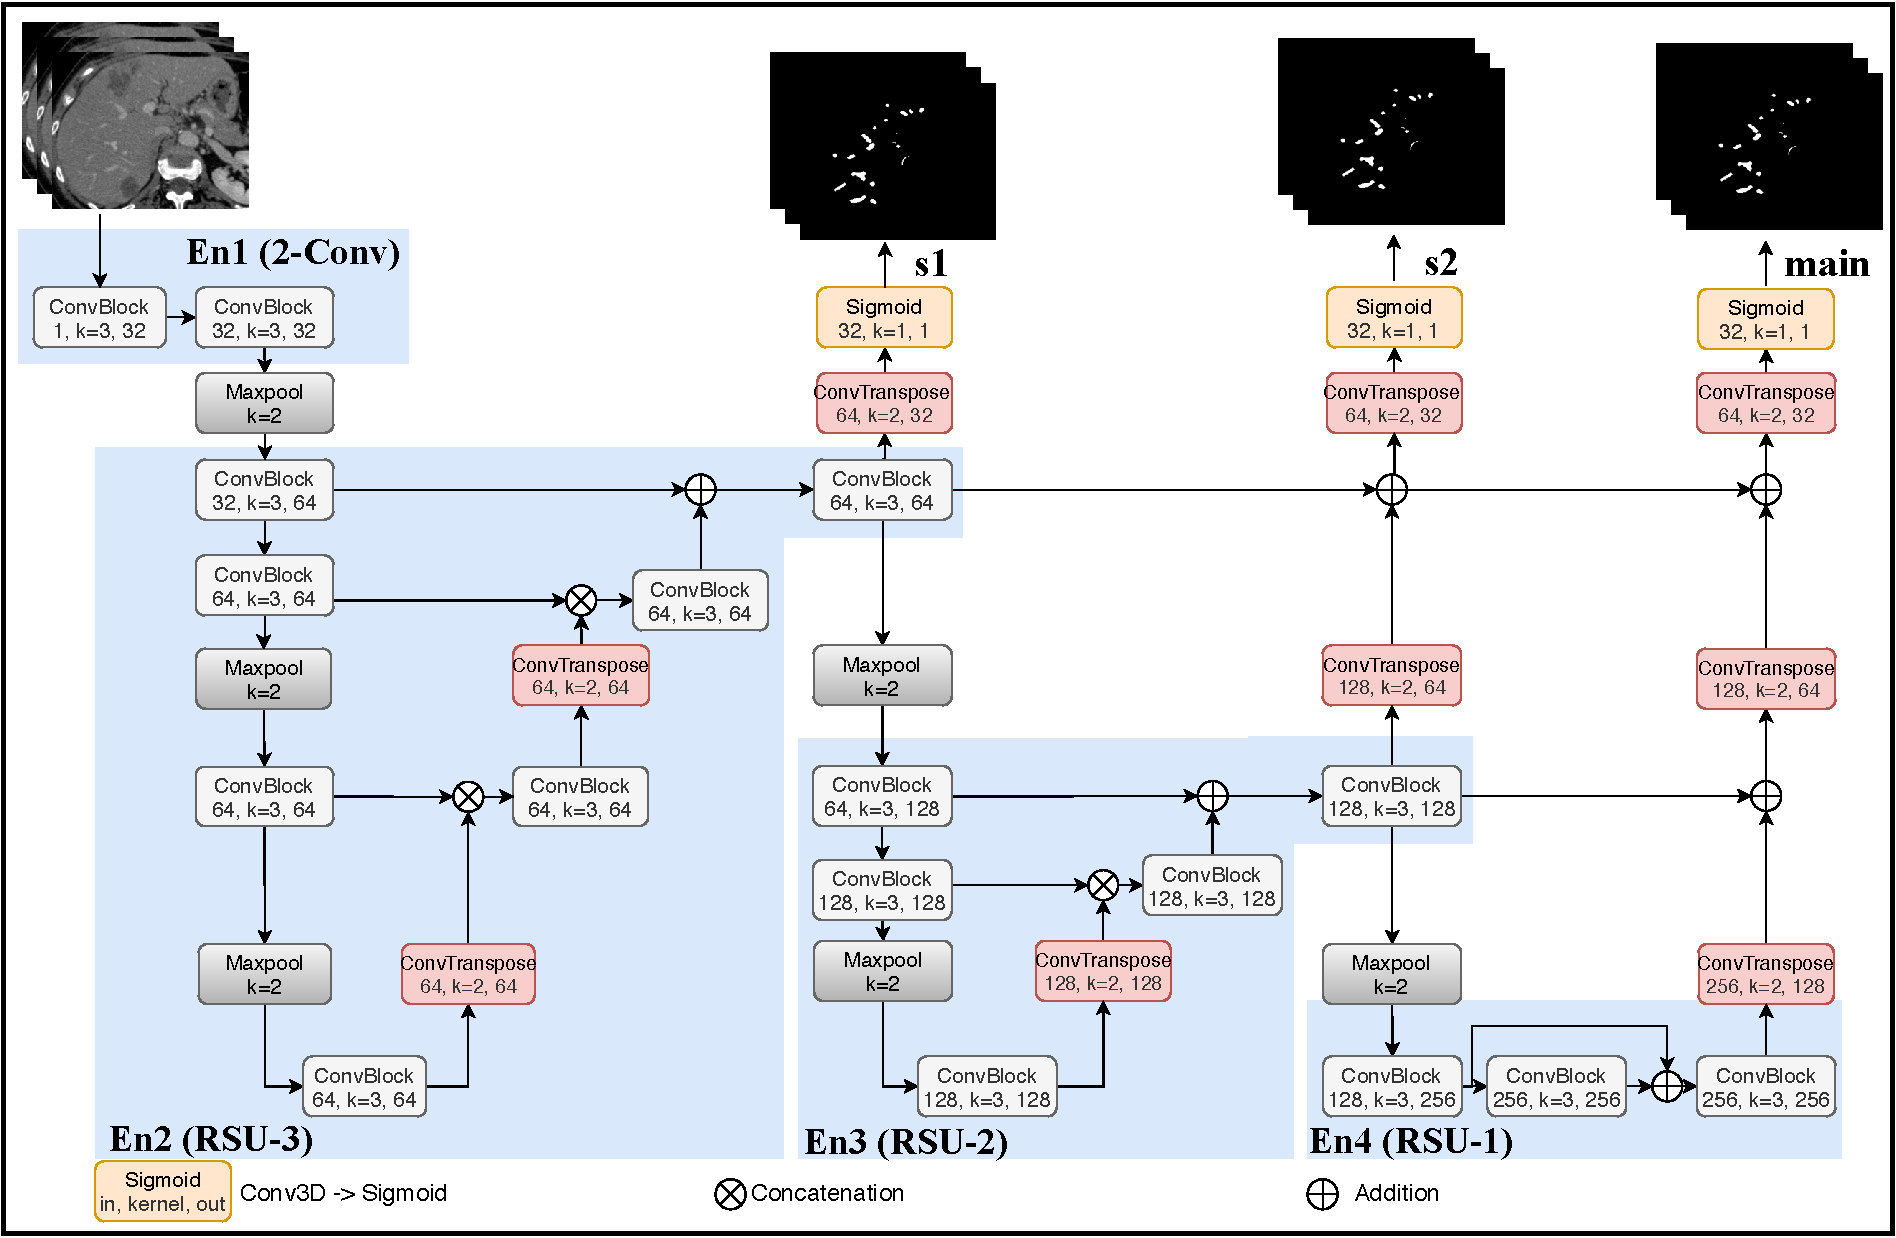
\includegraphics[scale=0.37]{figures/arch/u2net3d_arch.pdf}
		\end{figure}
	\end{frame}%------------------------------
	
\subsection{Hàm mục tiêu}
	\begin{frame}{Hàm mục tiêu}
	    \begin{align}
            Loss = \mu_{1}Loss_{s1} + \mu_{2}Loss_{s2} + \mu_{3}Loss_{main}
        \end{align}
        % Trong đó loss được tính dựa trên 2 công thức BCE hoặc Focal Loss:
        \begin{align}
            \mathrm{BCELoss}(q, p) &= -\log(q)\\
            \mathrm{FocalLoss}(q, p) &= -\alpha(1-q)^\gamma \log(q)\\
            \nonumber
            \alpha = \begin{cases} 
                            \alpha & \text{if } p = 1 \\
                            1-\alpha & \text{otherwise}
                        \end{cases}
            &\quad and \quad
            \mathrm{q} = \begin{cases} 
                    q & \text{if } p = 1 \\
                    1-q & \text{otherwise}
                  \end{cases}
        \end{align}
        \vspace{-8mm}\let\thefootnote\relax\footnote{\hspace{-3mm}\tiny *Các tham số $\mu_1=1, \mu_2=2, \mu_3=4$ đại diện cho mức độ quan trong của việc giám sát đặc trưng của các tầng.}
	\end{frame}

\section{Thí nghiệm và kết quả}
 \subsection{Tập dữ liệu}
	\begin{frame}{Tập dữ liệu}{Thông tin}
		\begin{block}{Các tập dữ liệu}
			\begin{enumerate}
				\item Segmentation of the Liver 2007 (SLIVER07).
				\item Liver Tumor Segmentation Challenge (LITS2017).
				\item 3D Image Reconstruction for Comparison of Algorithm Database (3DIRCADb).
			\end{enumerate}
		\end{block}
		\vspace{-2mm}
		\begin{figure}[h!]
			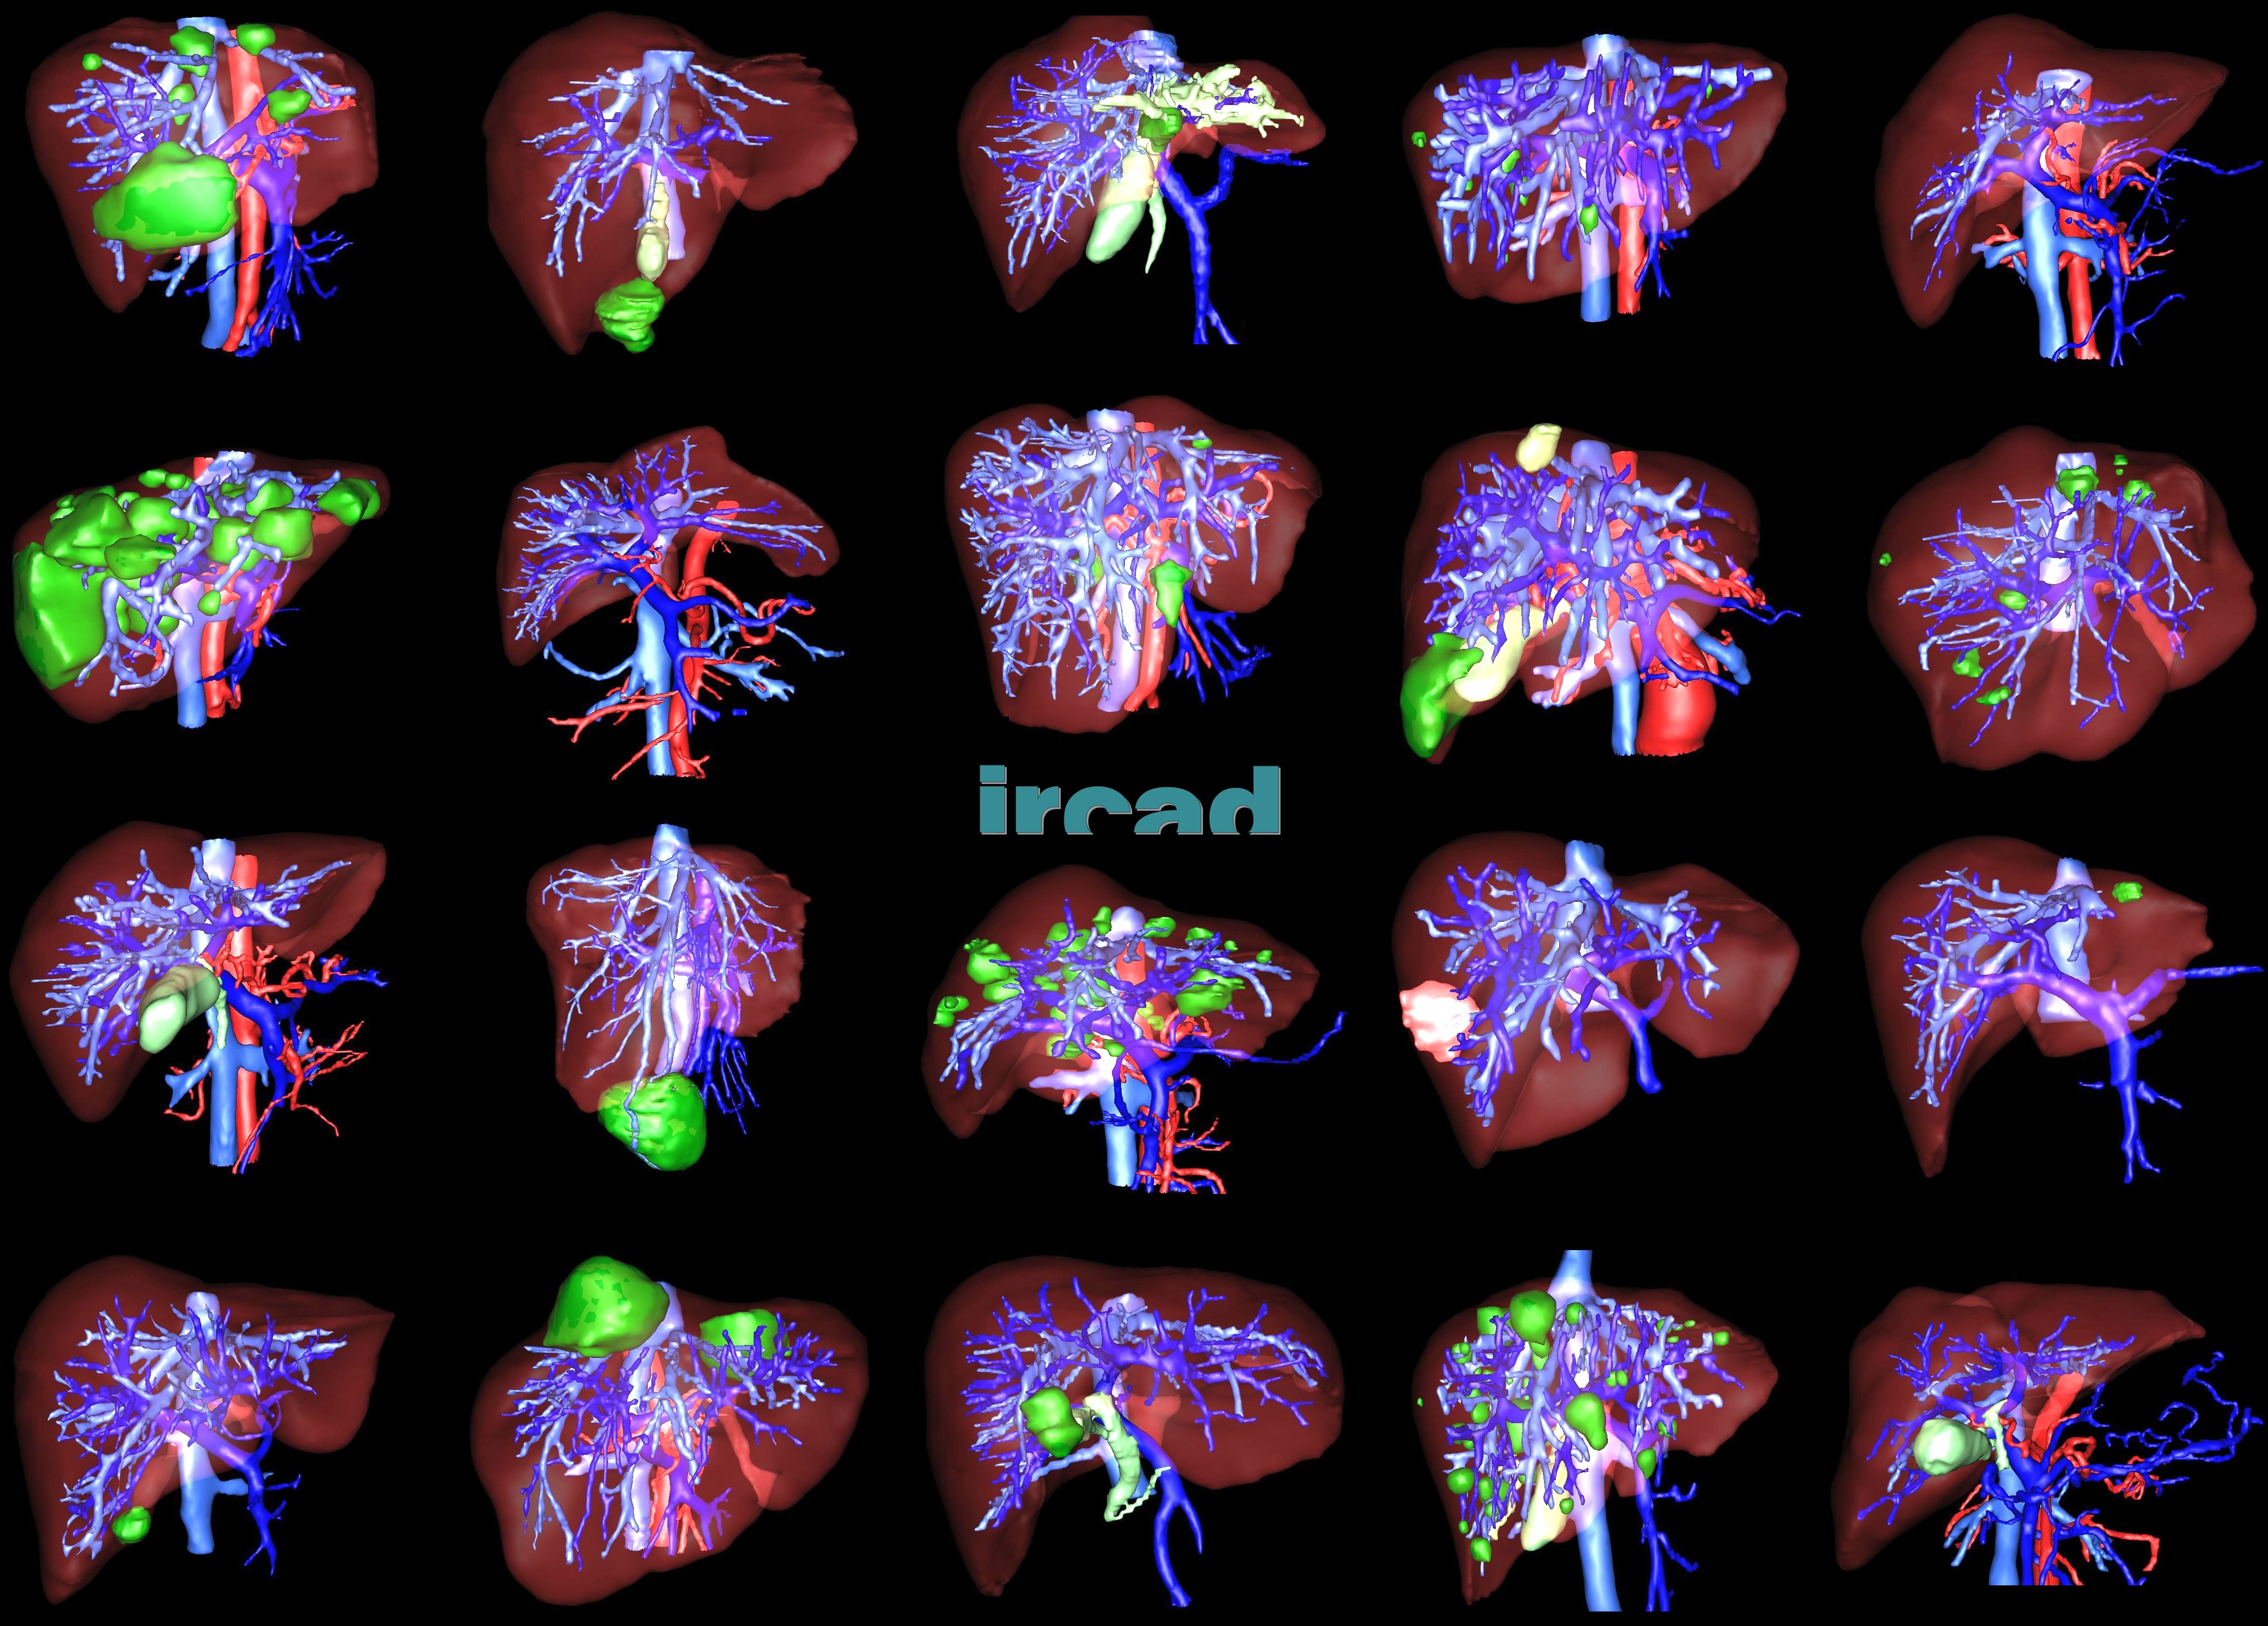
\includegraphics[height=.4\textheight]{figures/dataset/ircad_dataset}
			\vspace{-2mm}
			\caption{Ảnh trực quan tập dữ liệu \textit{3D-IRCADb-01}.}
		\end{figure}
		\footnotesource{\url{https://www.ircad.fr/research/3d-ircadb-01/}}
	\end{frame}
	
	\begin{frame}{Tập dữ liệu}{Tiền xử lý - Các bước tiền xử lý dữ liệu}
	    \vspace{-1.5cm}
		\begin{enumerate}
			\item Lấy mẫu dữ liệu đưa về cùng kích thước thực mỗi voxel: 1mm(W)$\times$1mm(H)$\times$1mm(D).
			\item Áp dụng ngưỡng lên dữ liệu.				
			\item Chuẩn hóa dữ liệu về khoảng giá trị [0, 1].
			\item Trích xuất thành phần gan (đối với bài toán mạch máu).
			\item Chia dữ liệu thành các khối 3D có kích thước nhỏ hơn.
			\item Tăng cường dữ liệu: xoay, biến dạng đàn hồi.
		\end{enumerate}
		
        \vspace{-0.5cm}
	\end{frame}
	
	\begin{frame}{Tập dữ liệu}{Tiền xử lý - Áp dụng ngưỡng và chuẩn hóa dữ liệu}
	    \vspace{-3mm}
	    \begin{minipage}[t]{.52\textwidth}
			\begin{figure}[h!]
		     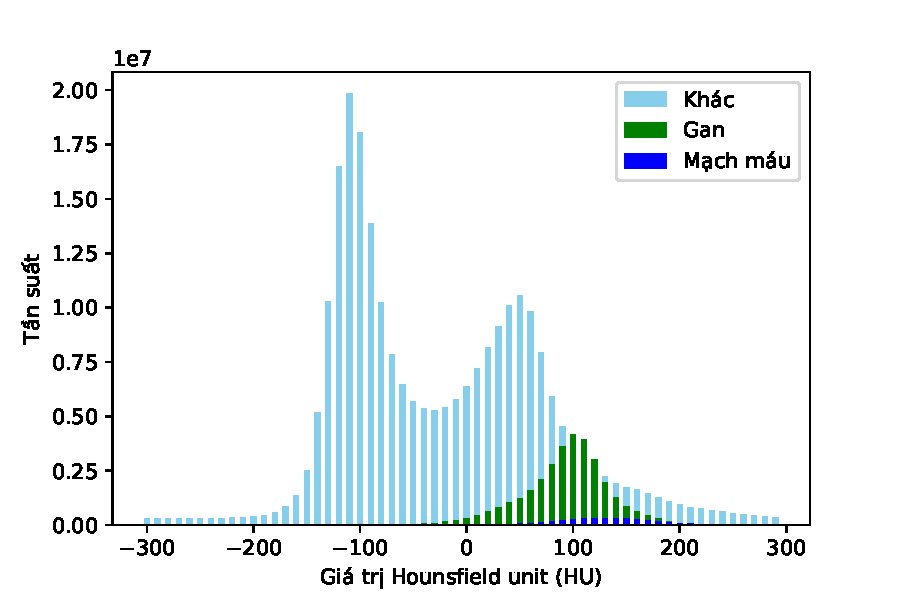
\includegraphics[scale=0.5]{figures/dataset/histogram_preprocess.pdf}
			    \caption{Phân phối giá trị Hounsfield Unit của gan, mạch máu và các bộ phận khác của tập dữ liệu 3Dircadb.}
		\end{figure}
	    \end{minipage}\hspace*{2mm}%
		\begin{minipage}[t]{.48\textwidth}
			\begin{enumerate}
			\setcounter{enumi}{1}
			\vspace{0.4cm}
			\item Áp dụng ngưỡng [min, max] lên dữ liệu.
			\begin{align}
                {P_{1x}} = \begin{cases} 
                    \mathrm{min} & \text{if}\ P_{1x} < min \\
                    \mathrm{max} & \text{if}\ P_{1x} > max \\
                    P_{1x}
                \end{cases}
            \end{align}
			\item Chuẩn hoá về khoảng giá trị [0, 1].
			\begin{equation}
			{P_2}_x=\dfrac{{P_1}_x - \mathrm{min}}{\mathrm{max} - \mathrm{min}}
			\end{equation}
		\end{enumerate}
	    \end{minipage}
	    
	    \vspace{-8mm}\let\thefootnote\relax\footnote{\hspace{-3mm}\tiny *Ngưỡng phù hợp sau khi phân tích các tập dữ liệu trong khoảng [-100, 400]}
 	\end{frame}
	
	\begin{frame}{Tập dữ liệu}{Tiền xử lý - Trích xuất thành phần gan}
	    \begin{figure}[h!]
			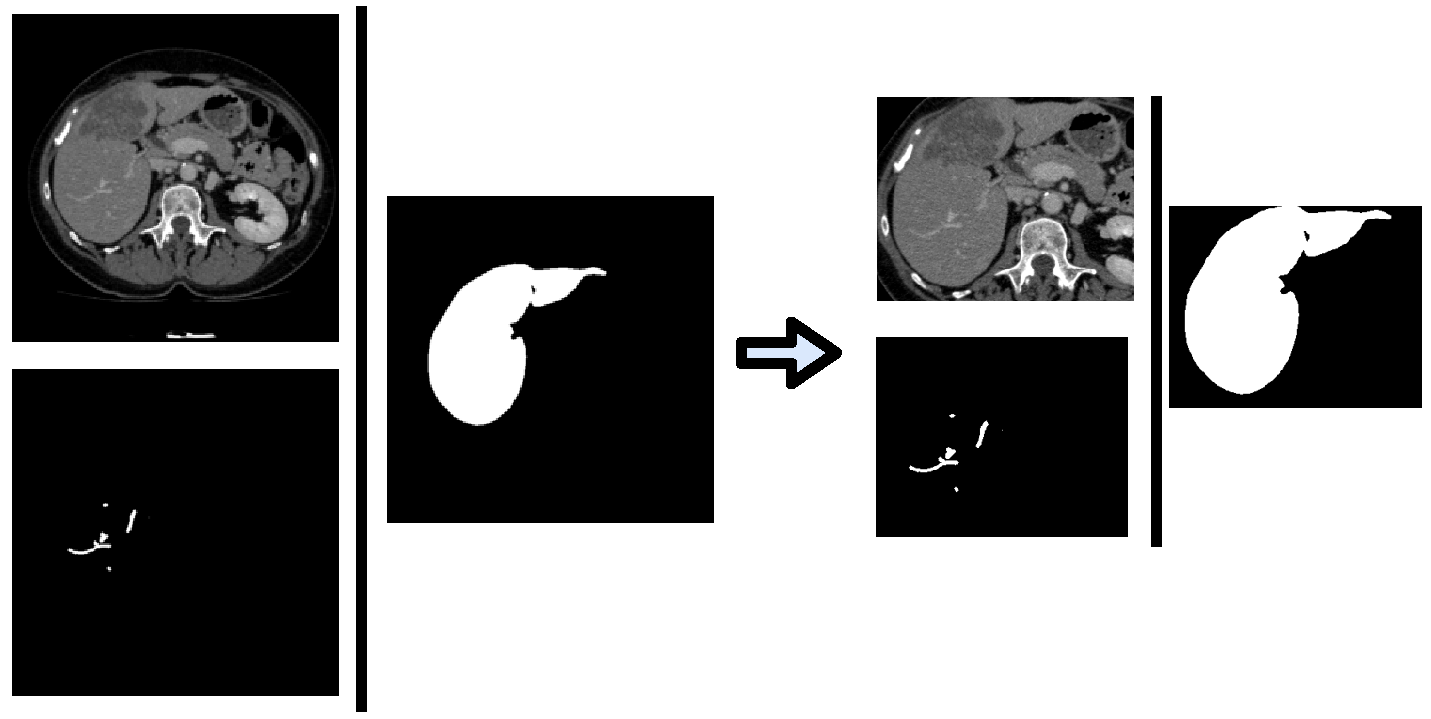
\includegraphics[height=.7\textheight]{figures/dataset/extract_liver.pdf}
			\vspace{-2mm}
			\caption{Trích xuất thành phần gan trong khối ảnh CT.}
		\end{figure}
	\end{frame}
	
	\begin{frame}{Tập dữ liệu}{Tiền xử lý - Trực quan hóa quy trình tiền xử lý}
	    \begin{figure}[h!]
			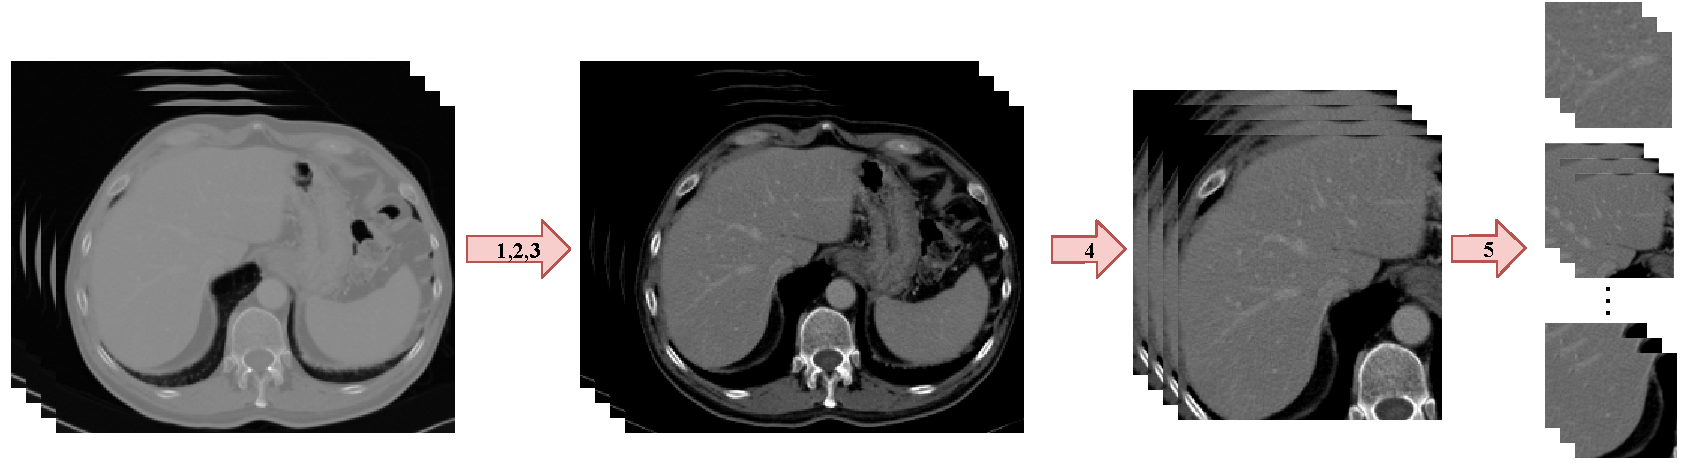
\includegraphics[scale=0.45]{Presentation_template/figures/dataset/preprocess_stage.pdf}
			\vspace{-2mm}
			\caption{Trực quan hóa quy trình tiền xử lý.}
		\end{figure}
	\end{frame}

	\begin{frame}{Tập dữ liệu}{Hậu xử lý}
		\vspace{5mm}
		\begin{block}{Hậu xử lý dữ liệu}
		Giải thuật đánh nhãn vùng liên thông.
		\end{block}
		\begin{figure}[h!]
		    \hspace{8mm}
			\begin{subfigure}[b]{0.3\textwidth}
				
\includegraphics[height=.4\textheight]{figures/liver_post_processing_before}
				\caption{}
				\label{fig:post_processing_before}
			\end{subfigure}
			\begin{subfigure}[b]{0.3\textwidth}
				
\includegraphics[height=.4\textheight]{figures/liver_post_processing_after}
				\caption{}
				\label{fig:post_processing_after}
			\end{subfigure}
			\vspace{-3mm}
			\caption{Loại bỏ các thành phần liên thông nhỏ. (\subref{fig:post_processing_before}) trước xử lý. (\subref{fig:post_processing_after}) sau xử lý.}
		\end{figure}
	\end{frame}
\subsection{Phương pháp đánh giá}
	\begin{frame}{Phương pháp đánh giá}{Độ đo}
	    \begin{minipage}[t]{.45\textwidth}
			\begin{align}
        		\mathrm{Dice} &= \mathrm{\dfrac{2TP}{2TP + FN + FP}} \\
        		\mathrm{Recall} &= \mathrm{\dfrac{TP}{TP + FN}} \\
        		\mathrm{Precision} &= \mathrm{\dfrac{TP}{TP + FP}}
            \end{align}
	    \end{minipage}\hspace*{2mm}%
		\begin{minipage}[t]{.45\textwidth}
		    \begin{align}
		    \mathrm{VOE} &= 1 - \mathrm{\dfrac{TP}{TP + FN + FP}} \\
			\mathrm{VD} &= \mathrm{\dfrac{FP - FN}{TP + FN}}
			\end{align}
	    \end{minipage}
		
		\vspace{-8mm}\let\thefootnote\relax\footnote{\hspace{-3mm}\tiny *Độ đo chính: Dice}
	\end{frame}

\subsection{Thí nghiệm}
    \begin{frame}{Thí nghiệm mô hình đề xuất U2net3d*}{Thí nghiệm trên gan}
	\begin{table}[H]
        \centering
        \begin{tabular}{c|c c c c c | c c}
        \Xhline{3\arrayrulewidth}
            \multirow{2}{*}{\textbf{STT}} & \multicolumn{5}{c|}{\textbf{Thông số mô hình}} & \multicolumn{2}{c}{\textbf{Tập kiểm thử}} \\
            & \textbf{En1} & \textbf{En2} & \textbf{En3} & \textbf{En4} & \textbf{En5} & \textbf{Dice} & \textbf{Recall} \\ 
            \hline
            \multirow{4}{*}{1} & \textbf{2-Conv} & \textbf{RSU-3} & \textbf{RSU-2} & \textbf{RSU-1} &  & \textbf{96.15} & 96.48 \\
                                          & I:1  & I:32 & I:64 & I:128 & \\ 
                                          & M:32 & M:64 & M:128 & M:256 & \\
                                          & O:32 & O:64 & O:128 & O:256 & \\
            \hline
            \multirow{4}{*}{2} & \textbf{2-Conv} & \textbf{RSU-4} & \textbf{RSU-3} & \textbf{RSU-2} &  & 94.85 & 96.22 \\
                                          & I:1  & I:32 & I:64 & I:128 & \\ 
                                          & M:32 & M:64 & M:128 & M:256 & \\
                                          & O:32 & O:64 & O:128 & O:256 & \\
            \hline
            \multirow{4}{*}{3} & \textbf{2-Conv} & \textbf{RSU-4} & \textbf{RSU-3} & \textbf{RSU-2} &  & 95.83 & \textbf{96.56} \\
                                          & I:1  & I:24 & I:48 & I:96 & \\ 
                                          & M:24 & M:48 & M:96 & M:192 & \\
                                          & O:24 & O:48 & O:96 & O:192 & \\
            \hline
    
        \Xhline{3\arrayrulewidth}
        \end{tabular}
        \caption{Thí nghiệm các siêu tham số mô hình U2net3d*.}
    \end{table}
	\end{frame}
	
	\begin{frame}{Thí nghiệm mô hình đề xuất U2net3d*}{Thí nghiệm trên gan}
	\begin{table}[H]
        \centering
        \begin{tabular}{c|c c c c c | c c}
        \Xhline{3\arrayrulewidth}
            \multirow{2}{*}{\textbf{STT}} & \multicolumn{5}{c|}{\textbf{Thông số mô hình}} & \multicolumn{2}{c}{\textbf{Tập kiểm thử}} \\
            & \textbf{En1} & \textbf{En2} & \textbf{En3} & \textbf{En4} & \textbf{En5} & \textbf{Dice} & \textbf{Recall} \\ 
            \hline
            \multirow{4}{*}{4} & \textbf{2-Conv} & \textbf{RSU-4} & \textbf{RSU-3} & \textbf{RSU-2} &  \textbf{RSU-1}  & 95.28 & 95.82 \\
                                          & I:1  & I:16 & I:32 & I:64  & I:128 \\ 
                                          & M:16 & M:32 & M:64 & M:128 & M:256 \\
                                          & O:16 & O:32 & O:64 & O:128 & O:256 \\
            \hline
            \multirow{4}{*}{5} & \textbf{2-Conv} & \textbf{RSU-5} & \textbf{RSU-4} & \textbf{RSU-3} &  \textbf{RSU-2}  & 93.94 & 94.35 \\
                                          & I:1  & I:12 & I:24 & I:48  & I:96 \\ 
                                          & M:12 & M:24 & M:48 & M:96 & M:192 \\
                                          & O:12 & O:24 & O:48 & O:96 & O:192 \\
            \hline
    
        \Xhline{3\arrayrulewidth}
        \end{tabular}
        \caption{Thí nghiệm các siêu tham số mô hình U2net3d*.}
    \end{table}
	\end{frame}
	
    \begin{frame}{Thí nghiệm mô hình đề xuất U2net3d*}{Thí nghiệm trên mạch máu}
    \vspace{3mm}
	\begin{table}[H]
        \centering
        \begin{tabular}{c|c c c c|c c}
        \Xhline{3\arrayrulewidth}
            \multirow{2}{*}{\textbf{STT}} & \multicolumn{4}{c|}{\textbf{Thông số mô hình}} & \multicolumn{2}{c}{\textbf{Tập kiểm thử}} \\
            & \textbf{En1} & \textbf{En2} & \textbf{En3} & \textbf{En4} & \textbf{Dice} & \textbf{Recall} \\ 
            \hline
            \multirow{4}{*}{1} & \textbf{RSU-4} & \textbf{RSU-3} & \textbf{RSU-2} & \textbf{RSU-1} & 58.50 & \textbf{75.12}\\
                                          & I:1  & I:32 & I:64 & I:128 \\ 
                                          & M:32 & M:32 & M:32 & M:32 \\
                                          & O:32 & O:64 & O:128 & O:256 \\
            \hline
            \multirow{4}{*}{2} & \textbf{RSU-4} & \textbf{RSU-3} & \textbf{RSU-2} & \textbf{RSU-1} & 61.14 & 68.86 \\
                                          & I:1  & I:32 & I:64 & I:128 \\ 
                                          & M:32 & M:64 & M:128 & M:256 \\
                                          & O:32 & O:64 & O:128 & O:256 \\
            \hline
            \multirow{4}{*}{3} & \textbf{RSU-4} & \textbf{RSU-3} & \textbf{RSU-2} & \textbf{RSU-1} & 61.73 & 70.78 \\
                                          & I:1  & I:32 & I:64 & I:128 \\ 
                                          & M:64 & M:64 & M:64 & M:64 \\
                                          & O:32 & O:64 & O:128 & O:256 \\
        \Xhline{3\arrayrulewidth}
        \end{tabular}
        \caption{Thí nghiệm các siêu tham số mô hình U2net3d*.}
    \end{table}
	\end{frame}
	
	\begin{frame}{Thí nghiệm mô hình đề xuất U2net3d*}{Thí nghiệm trên mạch máu}
	\vspace{3mm}
	\begin{table}[H]
        \centering
        \begin{tabular}{c|c c c c|c c}
        \Xhline{3\arrayrulewidth}
            \multirow{2}{*}{\textbf{STT}} & \multicolumn{4}{c|}{\textbf{Thông số mô hình}} & \multicolumn{2}{c}{\textbf{Tập kiểm thử}} \\
            & \textbf{En1} & \textbf{En2} & \textbf{En3} & \textbf{En4} & \textbf{Dice} & \textbf{Recall} \\ 
            \hline
            \multirow{4}{*}{4} & \textbf{RSU-2} & \textbf{RSU-2} & \textbf{RSU-2} & \textbf{RSU-2} & 60.84 & 67.84 \\
                                          & I:1  & I:32 & I:64 & I:128  \\ 
                                          & M:32 & M:64 & M:128 & M:256 \\
                                          & O:32 & O:64 & O:128 & O:256 \\
            \hline
            \multirow{4}{*}{5} & \textbf{2-Conv} & \textbf{RSU-3} & \textbf{RSU-2} & \textbf{RSU-1} & \textbf{63.08} & 70.31 \\
                                          & I:1  & I:32 & I:64 & I:128  \\ 
                                          & M:32 & M:64 & M:128 & M:256 \\
                                          & O:32 & O:64 & O:128 & O:256 \\
            \hline
            \multirow{4}{*}{6} & \textbf{2-Conv} & \textbf{RSU-3} & \textbf{RSU-2} & \textbf{RSU-1} & 62.12 & 64.36\\
                                          & I:1  & I:64  & I:128 & I:256 \\ 
                                          & M:64 & M:128 & M:256 & M:512 \\
                                          & O:64 & O:128 & O:256 & O:512 \\
        \Xhline{3\arrayrulewidth}
        \end{tabular}
        \caption{Thí nghiệm các siêu tham số mô hình U2net3d*.}
    \end{table}
	\end{frame}
	
\subsection{Đánh giá kết quả}
    \begin{frame}{Đánh giá kết quả}{So sánh với các công trình trước}
        \begin{table}[H]
        \renewcommand{\arraystretch}{1.1}
        \centering
        \begin{tabular}{c l c c c}
            \Xhline{2\arrayrulewidth}
            \multirow{2}{*}{\textbf{STT}} & \multirow{2}{*}{\textbf{Mô hình}} & \multicolumn{3}{c}{\textbf{Tập kiểm tra}} \\ \cline{3-5}
            & &  \textbf{Dice} & \textbf{Recall} & \textbf{Precision} \\ 
            \Xhline{2\arrayrulewidth}
            1   & Unet2D\small[\textcolor{blue}{1}]       & 41.17 & 60.05 & 31.32\\
            2   & Unet3D\small[\textcolor{blue}{2}]       & 56.29 & 44.27 & \textbf{73.97} \\
            3   & CNN3D\small[\textcolor{blue}{3}]        & 54.26 & 54.98 & 59.16 \\
            4   & U2net3D*     & \textbf{60.75} & \textbf{66.87} & 59.73 \\
            \Xhline{2\arrayrulewidth}
        \end{tabular}
        \caption{Kết quả phân đoạn mạch máu của các mô hình (\%).}
        \end{table}
        
    \vspace{-8mm}\let\thefootnote\relax\footnote{\hspace{-6mm}\scriptsize [\textcolor{blue}{1}] O. Ronneberger, P. Fischer, and T. Brox, “U-net: Convolutional networks for biomedical image segmentation,” MICCAI (2015)}
        
    \vspace{-8mm}\let\thefootnote\relax\footnote{\hspace{-6mm}\scriptsize [\textcolor{blue}{2}] L.H.Trong, N.V.Hung. “Phát hiện và xây dựng hệ thống mạch máu của gan từ ảnh chụp CT”, LVTN (2019)}
    
    \vspace{-8mm}\let\thefootnote\relax\footnote{\hspace{-6mm}\scriptsize [\textcolor{blue}{3}] Qi Dou, H.Chen. “3D Deeply Supervised Network for Automatic Liver Segmentation from CT Volumes”, CoRR (2016)}
    \end{frame}
    
    \begin{frame}{Đánh giá kết quả}{Đánh giá kết quả tập kiểm tra}
        \begin{table}[H]
        \renewcommand{\arraystretch}{1.1}
        \centering
        \begin{tabular}{c l c c c}
            \Xhline{2\arrayrulewidth}
            \multirow{2}{*}{\textbf{STT}} & \multirow{2}{*}{\textbf{Bệnh nhân}} & \multicolumn{3}{c}{\textbf{Tập kiểm tra}} \\ \cline{3-5}
            & &  \textbf{Dice} & \textbf{Recall} & \textbf{Precision} \\ 
            \Xhline{2\arrayrulewidth}
            1   & Bệnh nhân số 1 & 50.73 & \textbf{82.85} & 36.55\\
            2   & Bệnh nhân số 6 & 62.52 & 65.66 & 59.76 \\
            3   & Bệnh nhân số 11 & \textbf{68.79} & 64.09 & \textbf{74.23} \\
            \Xhline{2\arrayrulewidth}
        \end{tabular}
        \caption{Kết quả phân đoạn mạch máu chi tiết các bệnh nhân trong tập kiểm tra(\%).}
        \end{table}
    \end{frame}
    
    \begin{frame}{Đánh giá kết quả}{}
        \vspace{-0.3cm}
        \begin{figure}[H]
			\centering
		    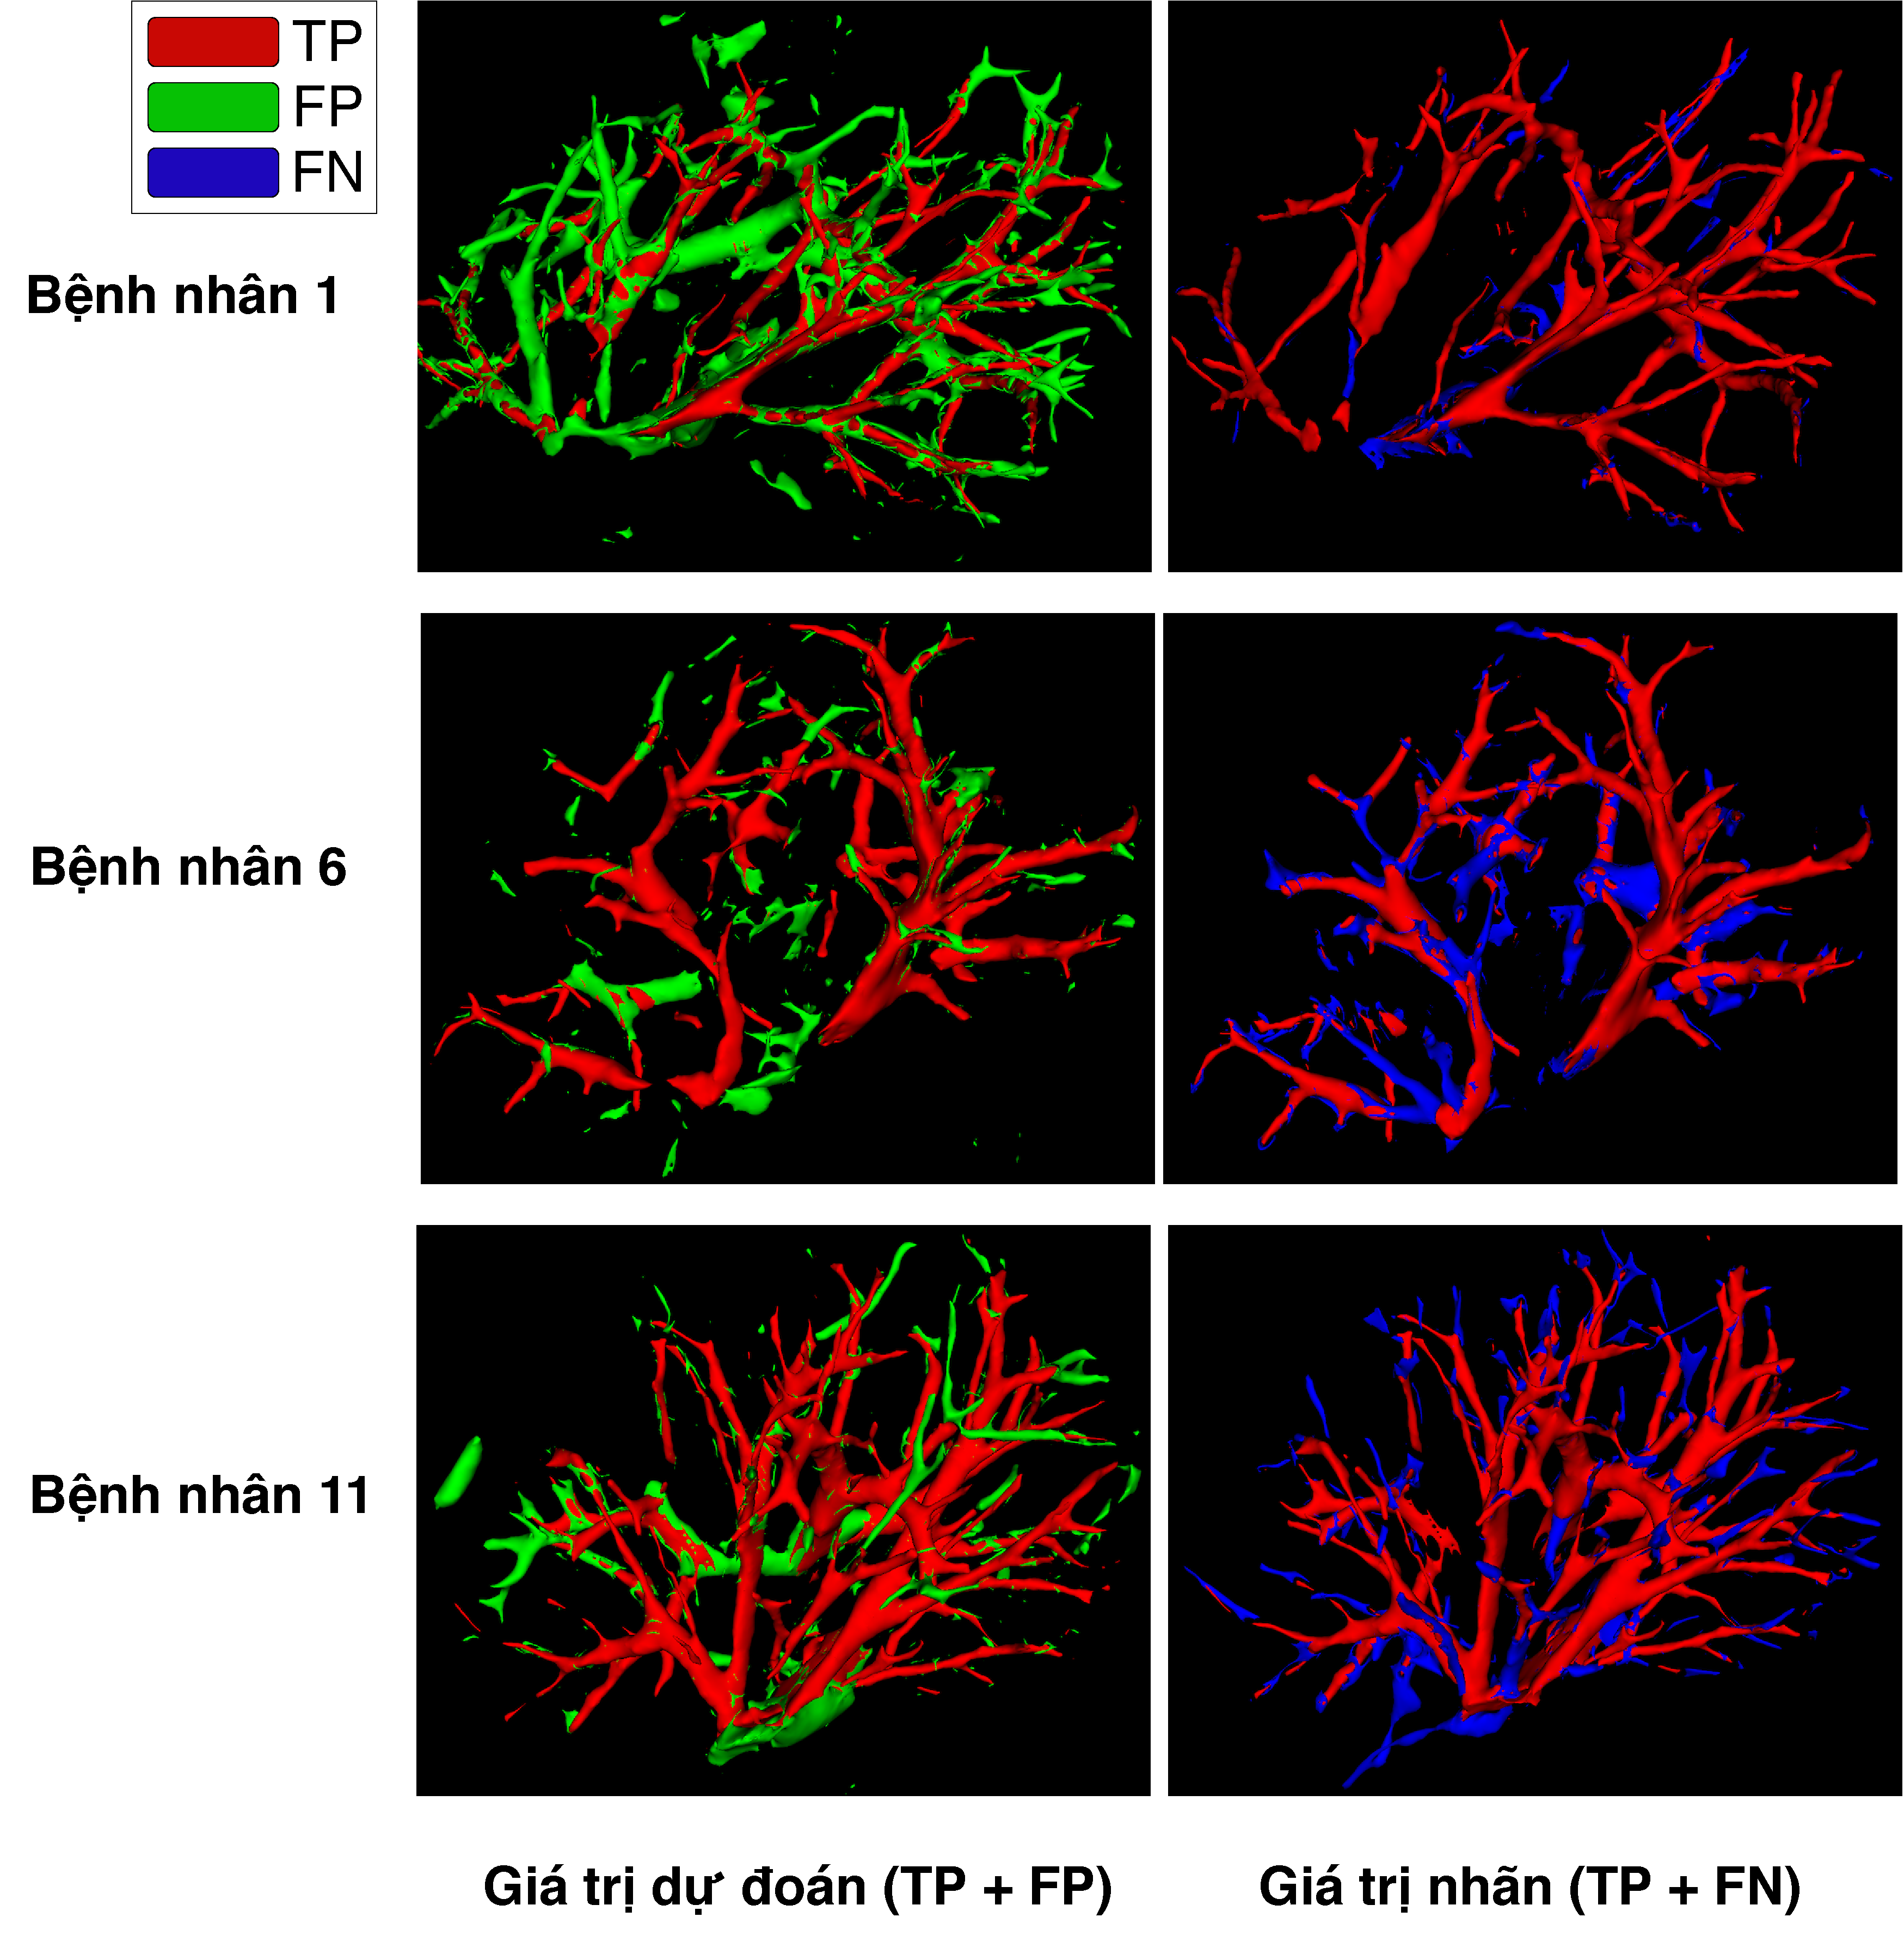
\includegraphics[height=0.9\textheight]{Presentation_template/figures/dataset/3d_vessel.pdf}
		\end{figure}
    \end{frame}
    
    \begin{frame}{Đánh giá kết quả}{So sánh với các công trình trước}
        \begin{table}[H]
        \centering
        \begin{tabular}{c c c c c c}
        \Xhline{3\arrayrulewidth}
        \multirow{2}{*}{\textbf{STT}} & \multirow{2}{*}{\textbf{Mô hình}} & \multicolumn{4}{c}{\textbf{Tập kiểm tra}} \\ \cline{3-6} 
        & &  \textbf{Dice} & \textbf{Recall} & \textbf{VOE} & \textbf{VD}\\ \hline
        1 & Unet3D\small[\textcolor{blue}{1}]   & 91.82   & 91.54     & 14.53  & 6.37  \\
        2 & CNN3D\small[\textcolor{blue}{2}]    & 95.17   & 94.42     & 9.11   & -1.64  \\
        3 & TLUnet3D\small[\textcolor{blue}{3}]        & 95.70   & \textbf{95.40}     & 8.16   & \textbf{-0.67}    \\
        4 & U2net3D* & \textbf{95.83}  & 95.29 & \textbf{7.9}  & -1.21 \\ 
        \Xhline{3\arrayrulewidth}
        \end{tabular}
        \caption{Kết quả phân đoạn gan của các mô hình (\%).}
        \end{table}
        
        \vspace{-8mm}\let\thefootnote\relax\footnote{\hspace{-6mm}\scriptsize [\textcolor{blue}{1}] L.H.Trong, N.V.Hung. “Phát hiện và xây dựng hệ thống mạch máu của gan từ ảnh chụp CT”, LVTN (2019)}
        
        \vspace{-8mm}\let\thefootnote\relax\footnote{\hspace{-6mm}\scriptsize [\textcolor{blue}{2}] Qi Dou, H.Chen. “3D Deeply Supervised Network for Automatic Liver Segmentation from CT Volumes”, CoRR (2016)}
        
        \vspace{-8mm}\let\thefootnote\relax\footnote{\hspace{-6mm}\scriptsize [\textcolor{blue}{3}] N.Q.Ha, T.Q.Phap, M.D.Tu. “Xây dựng mô hình gan từ ảnh chụp CT”, LVTN (2019)}
    \end{frame}
    
    \begin{frame}{Đánh giá kết quả}{Kết quả trực quan}
        \begin{figure}[H]
            \centering
            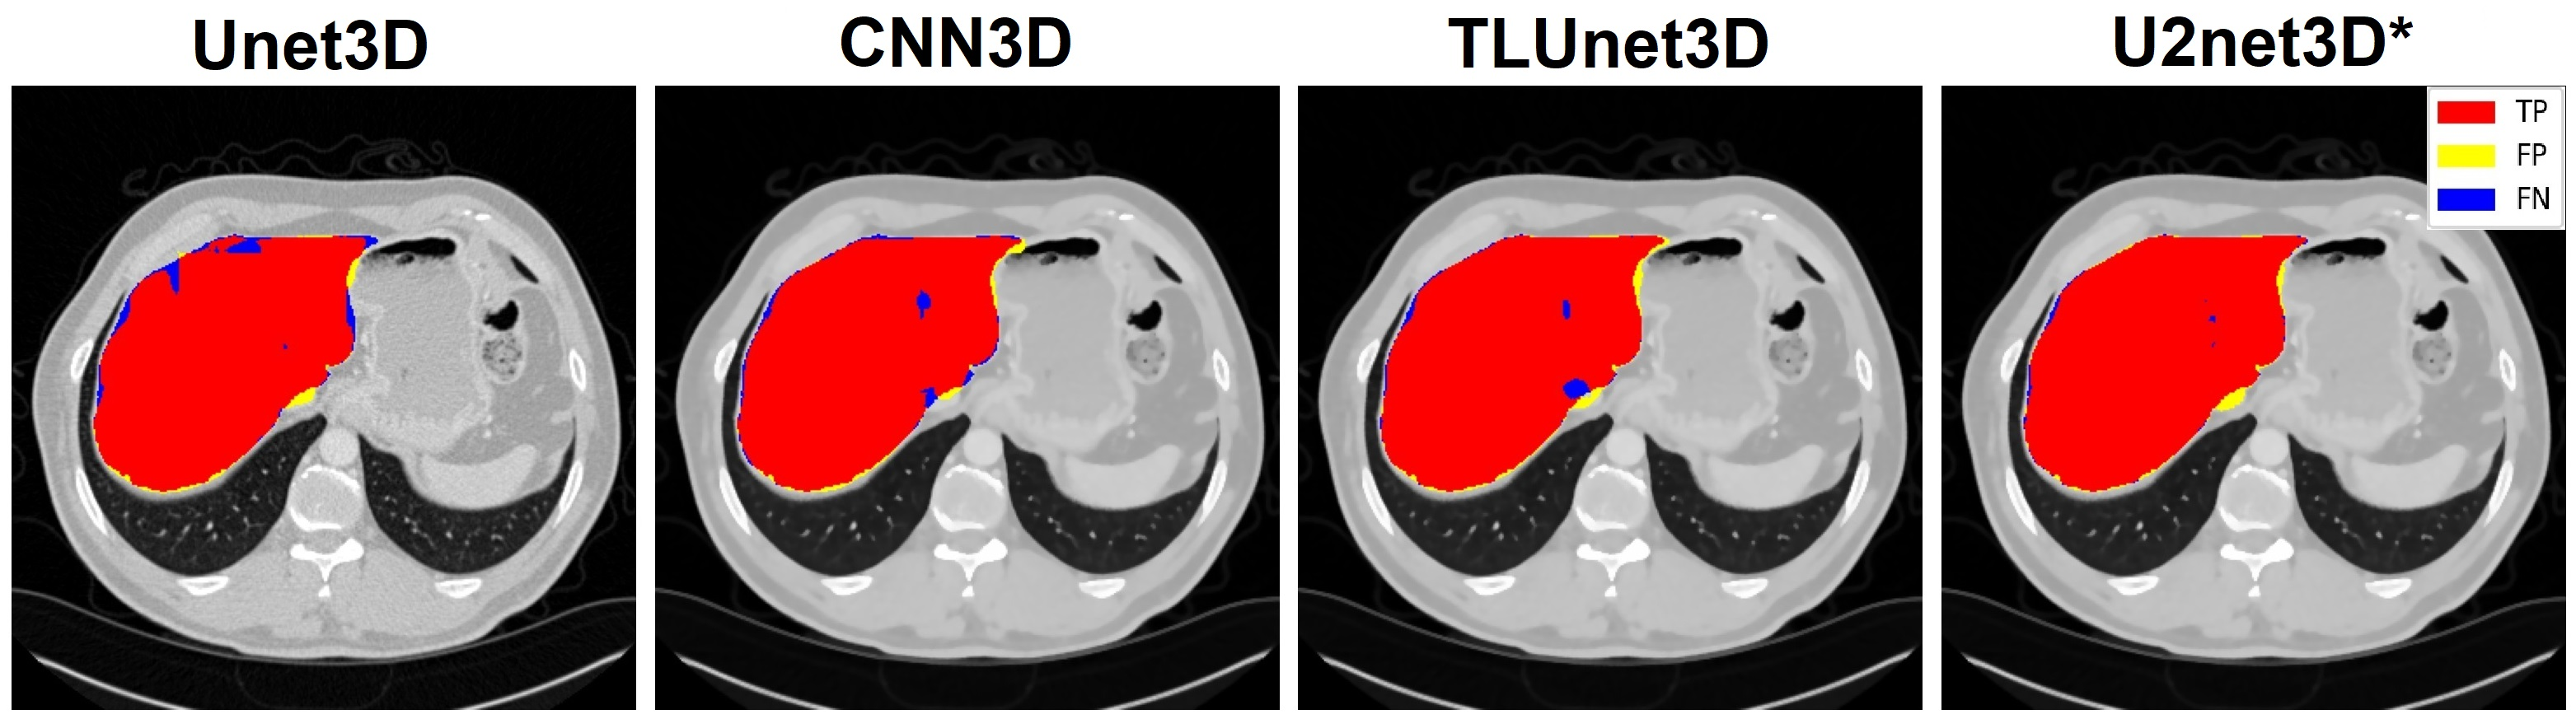
\includegraphics[width=\textwidth]{Presentation_template/figures/liver-result-legend.jpg}
            \caption{Kết quả dự đoán một mẫu dữ liệu trên tập Sliver07.}
        \end{figure}
    \end{frame}
    
\section{Hệ thống làm nhãn Data Annotation Tool}

\subsection{Mục tiêu hệ thống làm nhãn DAT}
    \begin{frame}{Mục tiêu hệ thống làm nhãn DAT}{}
		\begin{block}{Động lực}
			\begin{enumerate}
				\item Bài toán phân đoạn ảnh y khoa dùng mạng học sâu cần lượng lớn dữ liệu. 
				\item Việc gán nhãn dữ liệu ảnh y khoa cần một công cụ hỗ trợ hợp lý.
			\end{enumerate}
		\end{block}
		
		\begin{block}{Mục tiêu}
			\begin{enumerate}
				\item Cung cấp hệ thống DAT đáp ứng nhu cầu làm nhãn ảnh y khoa phục vụ việc huấn luyện mạng học sâu. 
			\end{enumerate}
		\end{block}
	\end{frame}	
    
\subsection{Kiến trúc hệ thống}
    \begin{frame}{Kiến trúc hệ thống}{Data Annotation Tool}
		\begin{figure}
			\centering
			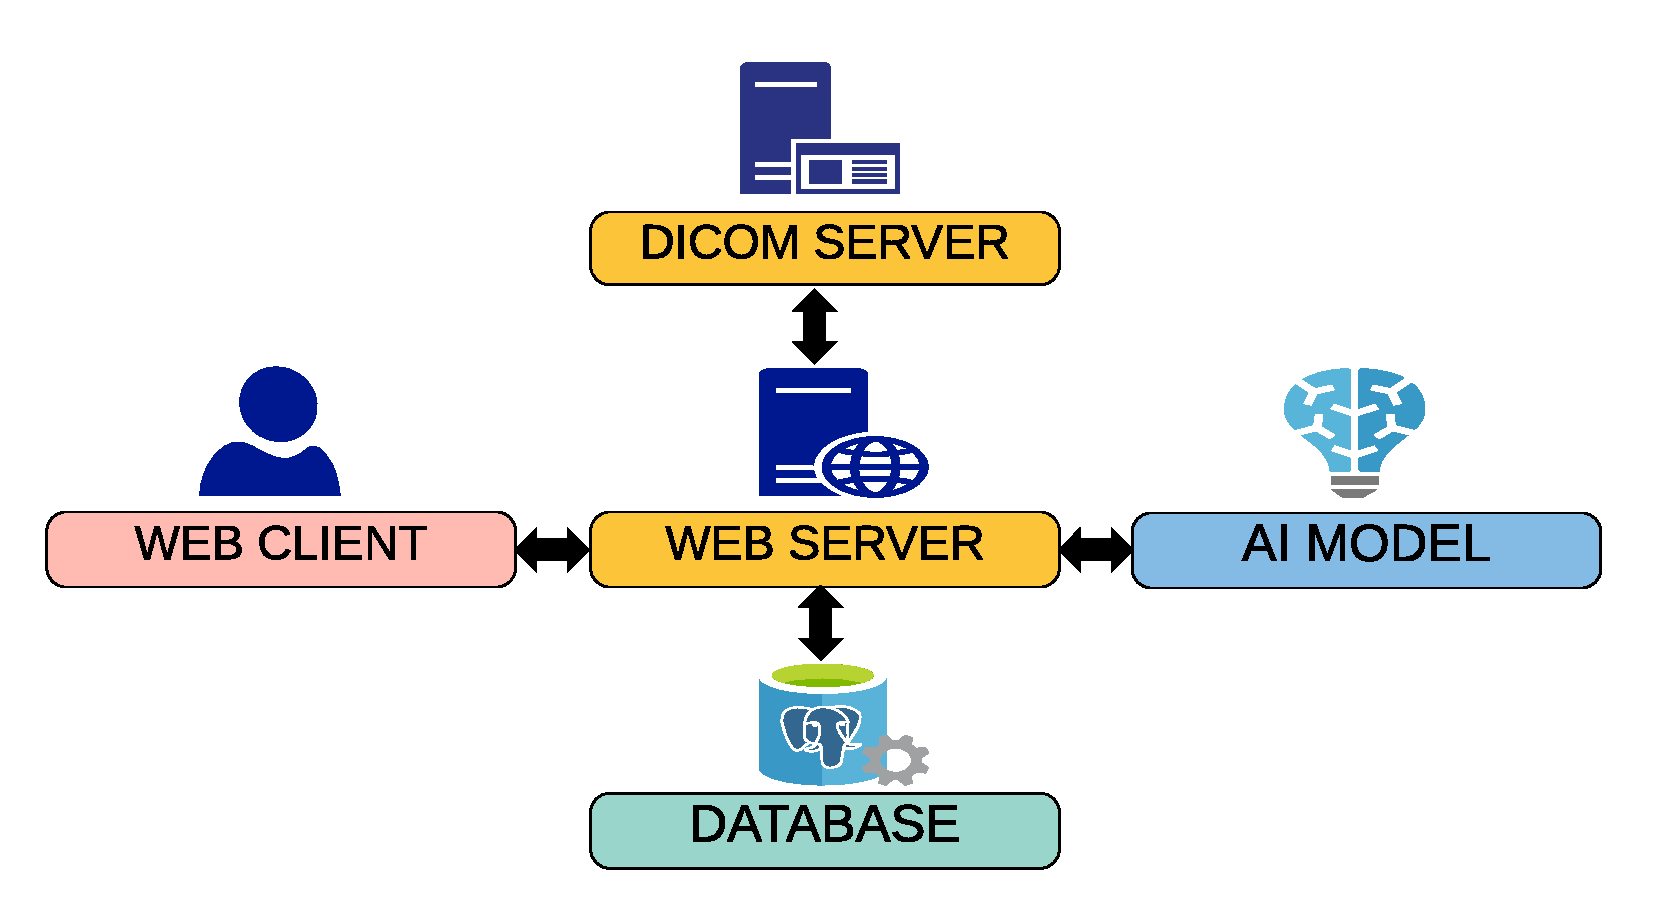
\includegraphics[width=0.9\linewidth]{Presentation_template/figures/DAT/mvt.pdf}
			\caption{Tổng quan hệ thống DAT}
		\end{figure}
	\end{frame}

\subsection{Giao diện ứng dụng}
    \begin{frame}{Giao diện ứng dụng}{Data Annotation Tool}
		\begin{figure}
			\centering
			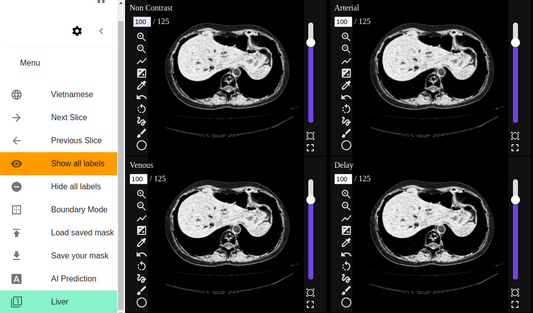
\includegraphics[width=0.78\linewidth]{Presentation_template/figures/DAT/dat_slide_user_ui.png}
			\caption{Giao diện làm nhãn}
		\end{figure}
	\end{frame}

\subsection{Làm nhãn với giải thuật tăng trưởng vùng}

\begin{frame}{Giải thuật tăng trưởng vùng}{Giới thiệu giải thuật}
% 		\begin{block}{Định nghĩa}
% 		\indent Là một kỹ thuật tuần tự dựa trên vùng để phân đoạn hình ảnh bằng cách tập hợp các pixel thành các vùng lớn hơn dựa trên các pixel hạt giống được xác định trước, tiêu chí phát triển và điều kiện dừng.
% 		\end{block}
		
		\begin{figure}[h!]
    	     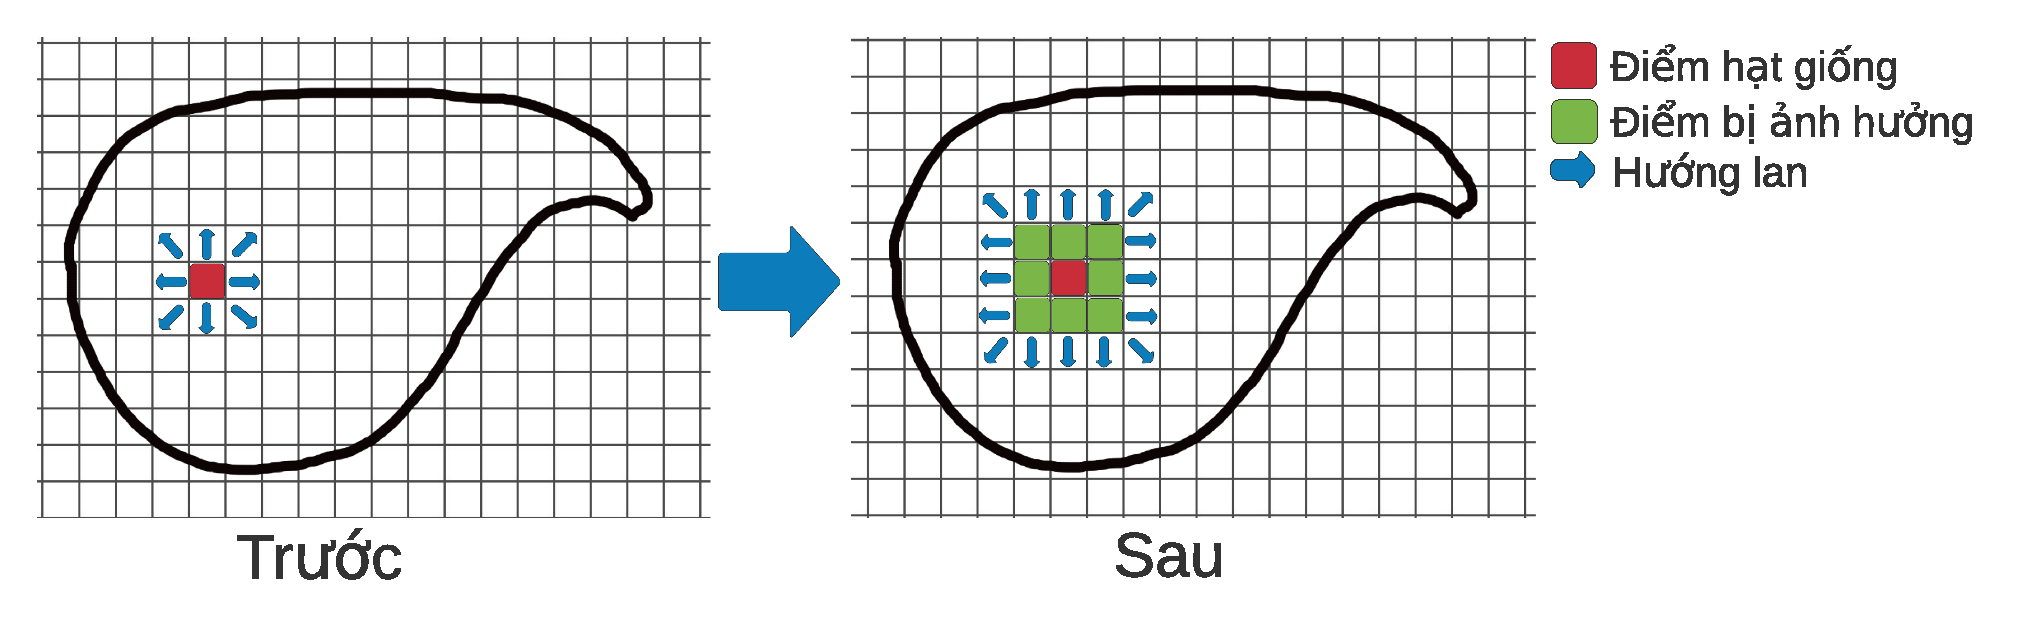
\includegraphics[width=0.98\textwidth]{Presentation_template/figures/DAT/dat_slide_region_growing_latest.pdf}
				\caption{Minh họa giải thuật tăng trưởng vùng}
		\end{figure}
\end{frame}

\begin{frame}{Giải thuật tăng trưởng vùng}{Ứng dụng giải thuật vào công cụ làm nhãn}
		\begin{block}{Ứng dụng vào thao tác làm nhãn}
			\begin{enumerate}
				\item Lấy ngưỡng giá trị Hounsfield. %để làm rõ đối tượng cần làm nhãn.
				\item Chọn điểm hạt giống.
				\item Tăng trưởng vùng theo mức xám. 
			\end{enumerate}
		\end{block}
		
		\begin{block}{Tiêu chí phát triển và điều kiện dừng}
		    \begin{enumerate}
		  %  \item Đặt một giá trị alpha có thể điều chỉnh, với mỗi pixel lân cận, nếu độ chênh lệch mức xám không vượt quá alpha thì được thêm vào vùng lan. 
				\item Độ chênh lệch mức xám không vượt quá alpha thì pixel được thêm vào vùng lan. 
				\item Độ chêch lệnh mức xám vượt quá alpha hoặc vị trí pixel ra ngoài hình ảnh thì dừng lại.
			\end{enumerate}
		\end{block}
		
\end{frame}

\begin{frame}{Làm nhãn với giải thuật tăng trưởng vùng}{Làm nhãn bán tự động}
		\begin{figure}[h!]
				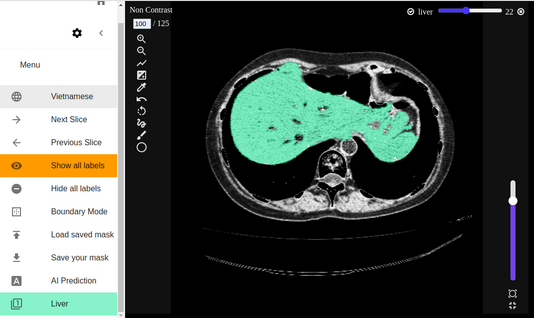
\includegraphics[width=0.8\textwidth]{Presentation_template/figures/DAT/dat_ui_labeling_region_growing.png}
				\caption{Tăng trưởng vùng theo mức xám trên ảnh DICOM}
		\end{figure}
\end{frame}

\subsection{Tích hợp dự đoán AI}

\begin{frame}{Tích hợp dự đoán AI}{Lãm nhãn bán tự động}
		\begin{figure}[h!]
				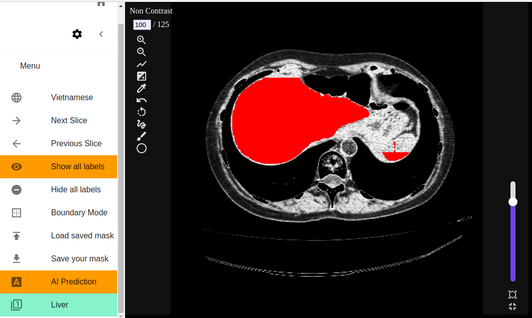
\includegraphics[width=0.8\textwidth]{Presentation_template/figures/DAT/dat_slide_labeling_with_ai.png}
				\caption{Dự đoán AI hỗ trợ làm nhãn ảnh DICOM}
		\end{figure}
\end{frame}
	
\subsection{Phần thừa kế và phần bổ sung}
	\begin{frame}{Phần thừa kế và phần bổ sung}{}
		\begin{block}{Tính năng thừa kế}
			\begin{enumerate}
			 %   \item Đăng nhập và xác thực người dùng.
			 %   \item Tải lên tập dữ liệu làm nhãn.
				% \item Cấu hình tập dữ liệu ảnh y khoa và chỉ định người dùng làm nhãn.
				% \item Hiện và ẩn nhãn.
				% \item Hiển thị đường biên.
				\item Lấy ngưỡng giá trị Hounsfield. %để làm rõ đối tượng cần làm nhãn.
				\item Vẽ bằng bút.
				\item Xóa bằng bút.
				\item Chọn vùng ROI (region of interest).
			\end{enumerate}
		\end{block}
		
		\begin{block}{Tính năng cải thiện và bổ sung}
			\begin{enumerate}
				\item Cải thiện giải thuật tăng trưởng vùng theo mức xám.
				\item Tích hợp dự đoán AI.
				% \item Quay về (undo).
				% \item Xóa toàn bộ nhãn.
				\item Vẽ nhãn tự do theo đường biên. 
				% \item Lưu nhãn đã làm.
				% \item Tải lên nhãn đã lưu.
				% \item Hỗ trợ ngôn ngữ tiếng Việt và tiếng Anh.
				% \item Phóng to, thu nhỏ, kéo thả hình ảnh khi làm nhãn.
				\item Đồng bộ nhãn giữa 4 thì.
				% \item Thanh cuộn để chuyển giữa các lát cắt trong quá trình làm nhãn.
			\end{enumerate}
		\end{block}
	\end{frame}	
	
% 	\begin{frame}{Phần thừa kế và phần bổ sung}{}
% 		\begin{block}{Tính năng cải thiện và bổ sung}
% 			\begin{enumerate}
% 				\item Cải thiện giải thuật tăng trưởng vùng theo mức xám.
% 				\item Tích hợp dự đoán AI.
% 				\item Quay về (undo).
% 				\item Xóa toàn bộ nhãn.
% 				\item Vẽ nhãn tự do theo đường biên. 
% 				\item Lưu nhãn đã làm.
% 				\item Tải lên nhãn đã lưu.
% 				\item Hỗ trợ ngôn ngữ tiếng Việt và tiếng Anh.
% 				\item Phóng to, thu nhỏ, kéo thả hình ảnh khi làm nhãn.
% 				\item Đồng bộ nhãn giữa 4 thì (thì không thuốc, thì động mạch, thì tĩnh mạch, thì muộn).
% 				\item Thanh cuộn để chuyển giữa các lát cắt trong quá trình làm nhãn.
% 			\end{enumerate}
% 		\end{block}
% 	\end{frame}	
	
\section{Tổng kết}
\subsection{Kết quả đạt được}
	\begin{frame}{Tổng kết}{Kết quả đạt được}
		\begin{block}{Kết quả đạt được}
			\begin{enumerate}
			    \item Mô hình phân đoạn mạch máu đề xuất đã cải thiện với hệ số Dice (\textbf{60.75\%}) so với các mô trình trước đó.
				\item Xây dựng thành công mô hình phân đoạn gan với độ chính xác tương đối tốt.
                \item Kế thừa và phát triển hệ thống làm nhãn ảnh y khoa.
			\end{enumerate}
		\end{block}
		\pause
		\begin{block}{Các đóng góp}
			\begin{enumerate}
				\item Việc áp dụng ý tưởng của mô hình trong lĩnh vực phát hiện đối tượng nổi bật nhất trong bài toán ảnh y khoa đạt được sự cải thiện.
				\item Phát triển thêm các tính năng hệ thống làm nhãn.
			\end{enumerate}
		\end{block}
	\end{frame}

\subsection{Hướng phát triển}
	\begin{frame}{Tổng kết}{Hướng phát triển}
		\begin{block}{Hướng phát triển}
			\begin{enumerate}
				\item Tích hợp phân đoạn đồng thời vừa gan vừa mạch máu cho toàn bộ ảnh CT.
				\item Phân đoạn nhiều cơ quan nội tạng khác nhau.
				\item Trực quan hóa dữ liệu dưới dạng mô hình 3D.
				\item Thêm tính năng tách riêng và thao tác độc lập trên từng phần nhãn.
				\item Cải thiện phần tải và hiển thị ảnh DICOM.
			\end{enumerate}
		\end{block}
	\end{frame}
	
% \subsection{Kế hoạch luận văn}
% 	\begin{frame}{Tổng kết}{Kế hoạch thực hiện luận văn}
% 		\vspace{-12mm}
% 		\begin{figure}[h!]
% 			\centering
% 			\setlength{\belowcaptionskip}{-1cm}
% 			\resizebox{\columnwidth}{!}{
% 				\begin{ganttchart}[
% 						canvas/.append style={fill=none, draw=black!15, line width=.75pt},
% 						hgrid style/.style={draw=black!15, line width=.75pt},
% 						vgrid={*1{draw=black!15, line width=.5pt}},
% 						x unit=.55cm,
% 						y unit title=1.2cm,
% 						y unit chart=.65cm,
% 						title/.style={draw=none, fill=none},
% 						title label font=\bfseries\footnotesize,
% 						title label node/.append style={below=7pt},
% 						include title in canvas=false,
% 						bar label font=\mdseries\small\color{black!70},
% 						bar label node/.append style={left=.1cm},
% 						bar/.append style={draw=none, fill=black!30},
% 						bar height=.7,
% 						group/.append style={draw=none, fill=black!60},
% 						% group incomplete/.append style={fill=groupblue},
% 						group left shift=0,
% 						group right shift=0,
% 						group height=.3,
% 						group peaks tip position=0,
% 						group label node/.append style={left=.1cm},
% 					]{1}{15}
% 					\gantttitle[
% 						title label node/.append style={below left=4pt and 3pt}
% 					]{TUẦN:}{0}
% 					\gantttitlelist{1,...,15}{1} \\
% 					\Dganttbar{\textbf{1.} Viết báo cáo Luận văn}{Hùng, Trọng}{1}{15}\\
% 					\Dganttbar{\textbf{2.} Tiền xử lý tập dữ liệu}{\hspace{12mm}Hùng, Trọng}{1}{1}\\
% 					\Dganttbar{\textbf{3.} Huấn luyện mô hình U-Net}{Hùng}{2}{5}\\
% 					\Dganttbar{\textbf{4.} Huấn luyện mô hình DeepVesselNet}{Trọng}{2}{5}\\
% 					\Dganttbar{\textbf{5.} Tổng kết, đánh giá, đề xuất mô hình}{\hspace{7mm}Hùng, Trọng}{6}{7}\\
% 					\Dganttbar{\textbf{6.} Huấn luyện, đánh giá mô hình}{Trọng}{8}{12}\\
% 					\Dganttbar{\textbf{7.} Trực quan hoá kết quả thí nghiệm}{Hùng}{8}{9}\\
% 					\Dganttbar{\textbf{8.} Hậu xử lý kết quả phân đoạn}{Hùng}{10}{12}\\
% 					\Dganttbar{\textbf{9.} Xây dựng bài thuyết trình}{\hspace{7mm}Hùng, Trọng}{13}{14}\\
% 					\Dganttbar{\textbf{10.} Chuẩn bị poster}{\hspace{13mm}Hùng, Trọng}{15}{15}
% 				\end{ganttchart}
% 			}
% 			\caption{Kế hoạch thực hiện luận văn.}
% 			\label{fig:ke_hoach_thuc_hien_luan_van}
% 		\end{figure}
% 	\end{frame}

\setcounter{section}{0}
\appendix
	\begin{frame}[noframenumbering]
		\begin{minipage}[c][\textheight][c]{\textwidth}%
			\centering
			\LARGE
			\textcolor{blue}{\textbf{Cảm ơn thầy cô và các bạn đã lắng nghe!}}
		\end{minipage}%
	\end{frame}
	
	\begin{frame}[noframenumbering]{Thí nghiệm mô hình Unet3D}{Thí nghiệm trên gan}
        \begin{table}[H]
            \centering
            \resizebox{\columnwidth}{!}{
            \begin{tabular}{c|c|c|c|c|c|c}
            \Xhline{3\arrayrulewidth}
            \multirow{2}{*}{\textbf{STT}} & \multirow{2}{*}{\textbf{Thí nghiệm}} & \multirow{2}{*}{\textbf{\begin{tabular}[c]{@{}l@{}}Kích thước \\ dữ liệu\end{tabular}}} & \multirow{2}{*}{\textbf{\begin{tabular}[c]{@{}l@{}}Độ sâu \\ mô hình \end{tabular}}} & \multirow{2}{*}{\textbf{\begin{tabular}[c]{@{}l@{}}Tăng cường\\ dữ liệu\end{tabular}}} & \multicolumn{2}{c}{\textbf{Tập kiểm thử}} \\ \cline{6-7} 
            & & &  & & \textbf{Dice}  & \textbf{Recall}  \\ \hline
            1 & \multirow{4}{*}{\begin{tabular}[c]{@{}l@{}}Kích thước \\ dữ liệu\end{tabular}} & $64^3$ & \multirow{4}{*}{3} & \multirow{6}{*}{Không} & 71.69  & 88.66   \\ \cline{1-1} \cline{3-3} \cline{6-7} 
            2 & & $96^3$ & &                                                                                        & 83.49            & 89.93            \\ \cline{1-1} \cline{3-3} \cline{6-7} 
            3                             &                                                                                & $128^3$                                                                                     &                                                                                               &                                                                                        & 80.12            & 85.81            \\ \cline{1-1} \cline{3-3} \cline{6-7} 
            4                             &                                                                                & $160^3$                                                                                     &                                                                                               &                                                                                        & 80.94            & 87.81            \\ \cline{1-4} \cline{6-7} 
            5                             & \multirow{2}{*}{\begin{tabular}[c]{@{}l@{}}Độ sâu \\ mô hình\end{tabular}}     & \multirow{3}{*}{$96^3$}                                                                     & 4                                                                                             &                                                                                        & 88.17            & 90.49            \\ \cline{1-1} \cline{4-4} \cline{6-7} 
            6 & &  & 5 &                                                                                        & 88.09            & \textbf{94.20}   \\ \cline{1-2} \cline{4-7} 
            7                             & \begin{tabular}[c]{@{}l@{}}Tăng cường \\ dữ liệu\end{tabular}                  &                                                                                         & 4                                                                                             & Có                                                                                     & \textbf{90.67}   & 91.52            \\ 
            \Xhline{3\arrayrulewidth}
            \end{tabular}}
            \caption*{Kết quả thí nghiệm mô hình Unet3D trên gan.}
        \end{table}

	\end{frame}
	
    \begin{frame}[noframenumbering]{Thí nghiệm mô hình CNN3D}{Thí nghiệm trên gan}
        \begin{table}[H]
            \renewcommand{\arraystretch}{1.2}
            \centering
            \begin{tabular}{c|c|c|c|c}
                \Xhline{3\arrayrulewidth}
                \multirow{2}{*}{\textbf{Thí nghiệm}} & \multicolumn{4}{c}{\textbf{Tập kiểm tra}}\\
                \cline{2-5} 
                & \textbf{Dice} (\%) & \textbf{Recall} (\%) & \textbf{VOE} (\%) & \textbf{VD} (\%) \\ 
                \hline
                CNN 3D          & 94.61              & 94.40                & 10.11    & \textbf{-0.47}\\ 
                \hline
                CNN 3D + hậu xử lý  & \textbf{95.17}   & \textbf{94.42} & \textbf{9.11}   & -1.64       \\ 
                \Xhline{3\arrayrulewidth}
            \end{tabular}
            \caption*{Kết quả thí nghiệm mô hình CNN3D trên gan.}
        \end{table}
    \end{frame}
    
    \begin{frame}[noframenumbering]{Thí nghiệm mô hình U2net3D*}{Thí nghiệm trên gan}
        \begin{table}[H]
            \renewcommand{\arraystretch}{1.1}
            \centering
            \begin{tabular}{c|c|c|c|c}
            \Xhline{3\arrayrulewidth}
            \multirow{2}{*}{\textbf{Thí nghiệm}} & \multicolumn{4}{c}{\textbf{Tập kiểm tra}}                             \\ \cline{2-5} 
            & \textbf{Dice} (\%) & \textbf{Recall} (\%) & \textbf{VOE} (\%) & \textbf{VD} (\%) \\ \hline
            U2net3D*      & 95.28     & 95.29     & 8.92     & \textbf{-0.04}    \\ \hline
            U2net3D* + hậu xử lý & \textbf{95.83}       & 95.29     & \textbf{7.9}   & -1.21       \\ 
            \Xhline{3\arrayrulewidth}
            \end{tabular}
            \caption*{Kết quả thí nghiệm mô hình U2net3D* trên gan.}
        \end{table}
    \end{frame}
	
	\begin{frame}[noframenumbering]{Phân tích tập dữ liệu}
	    \vspace{-0.35cm}
	    \begin{figure}[H]
        	\begin{center}
        		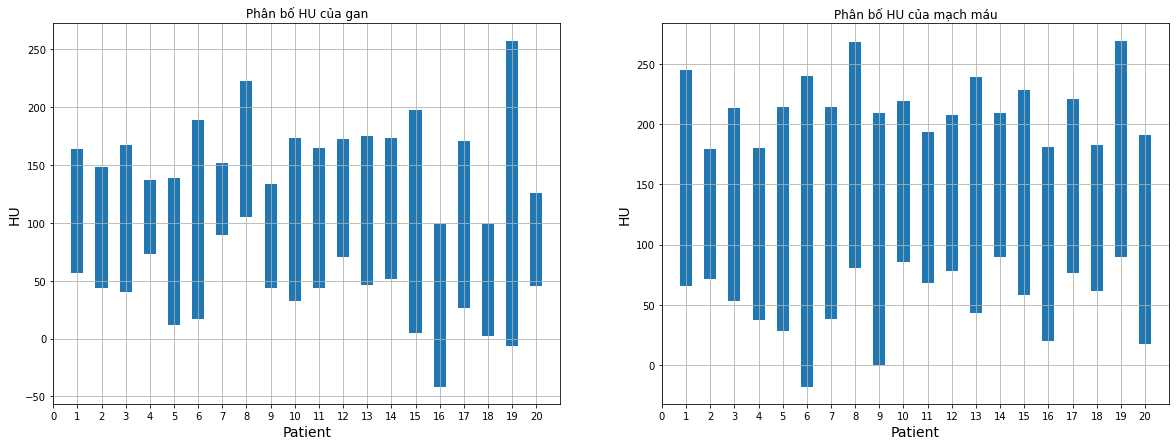
\includegraphics[scale=0.26]{Presentation_template/figures/dataset/hu_dist.png}
        % 		\caption{Phân bố giá trị HU từng bệnh nhân.}
        	\end{center}
        	\vspace{-0.3cm}
        	\begin{center}
        		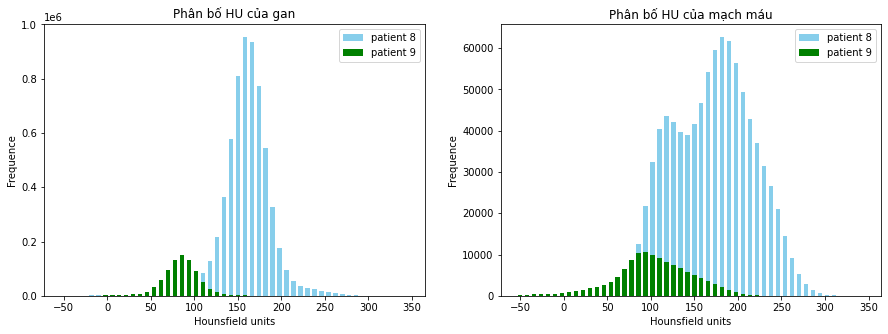
\includegraphics[scale=0.35]{Presentation_template/figures/dataset/compare_2patient.png}
        % 		\caption{So sánh phân bố HU của 2 bệnh nhân số 8 và số 9.}
        	\end{center}
        \end{figure}
	\end{frame}
	
	\begin{frame}[noframenumbering]{Chuẩn bị dữ liệu huấn luyện}
	    \begin{table}[H]
            \centering
            \begin{tabular}{|c|l|l|l|l|c|}
            \hline
            \multicolumn{1}{|c|}{\multirow{2}{*}{\textbf{STT}}} & \multicolumn{1}{c|}{\multirow{2}{*}{\textbf{Tập}}} & \multicolumn{3}{c|}{\textbf{Phân phối giá trị trung bình HU}}       & \multirow{2}{*}{\textbf{Tổng}} \\ \cline{3-5}
            \multicolumn{1}{|c|}{}                     & \multicolumn{1}{c|}{}                     & \textless{}125 & {[}125 , 150{]}        & \textgreater 150 &                       \\ \hline
            0 & Huấn luyện   & 5, 16, 9, 18, 20  & 2, 3, 7, 12, 13, 14, 15 & 8, 10    & 14                    \\ \hline
            1 & Kiểm thử     & 4             & 17                     & 19          & 3                     \\ \hline
            2 & Kiểm tra     & 6             & 11                     & 1           & 3                     \\ \hline
            \end{tabular}
            \caption*{\textcolor{blue}{\textbf{Bảng B.1:}}Bảng phân chia các bệnh nhân thành các tập dữ liệu cho mạch máu.}
        \end{table}
	\end{frame}
	
	\begin{frame}[noframenumbering]{Phân tích tập dữ liệu}
	    \vspace{-0.3cm}
	    \begin{figure}[H]
    	    \centering
        	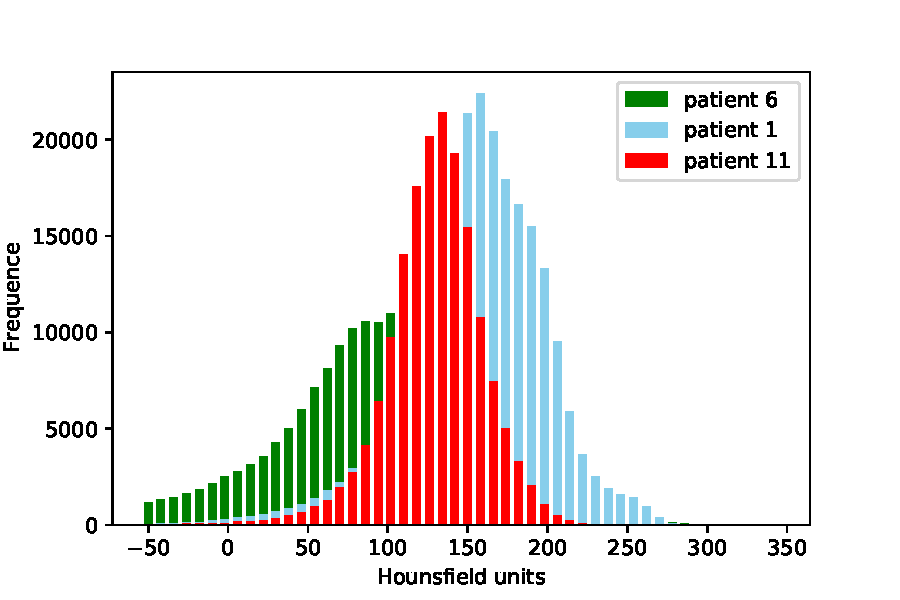
\includegraphics[scale=0.7]{Presentation_template/figures/dataset/test_hist.pdf}
        	\caption*{\textcolor{blue}{\textbf{Hình A.1:}} Phân bố HU của từng bệnh nhân trên tập kiểm tra.}
        \end{figure}
	\end{frame}
	
	\begin{frame}[noframenumbering]{Hàm mục tiêu - Focal Loss}
	    \vspace{-0.8cm}
        \begin{figure}[H]
            \centering
            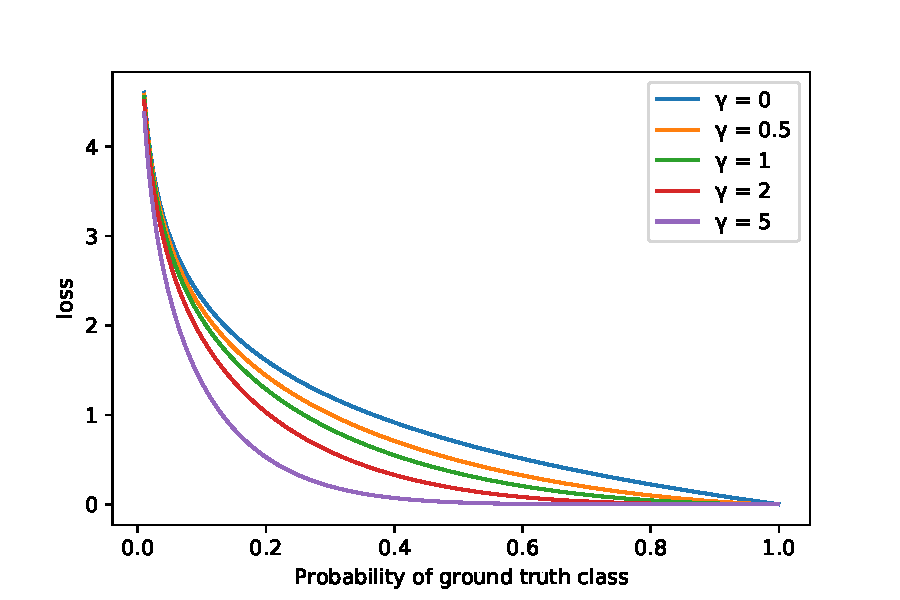
\includegraphics[width=10cm]{Presentation_template/figures/focal.pdf}
            \caption*{\textcolor{blue}{\textbf{Hình A.1:}}Sự ảnh hưởng của trọng số $\gamma$ đối với hàm focal loss $\mathrm{FL(q)=-(1-q)^\gamma \mathrm{log}(q)}$ }
        \end{figure}
        \footnotesource{Tsung{-}Yi Lin, Priya Goyal, Ross B. Girshick, Kaiming He, Piotr Doll ``Focal Loss for Dense Object Detection'', 2017} 
	\end{frame}    
	
	\begin{frame}[noframenumbering]{Thí nghiệm mô hình Unet3D - mạch máu}
	    \begin{table}[H]
            \centering
            \begin{tabular}{c|c|c|c|c}
            \Xhline{3\arrayrulewidth}
            \multirow{2}{*}{\textbf{Mô hình}} & \multirow{2}{*}{\textbf{Độ sâu}} & \multicolumn{2}{c|}{\textbf{Tập kiểm tra}} & \multirow{2}{*}{\textbf{Số lượng tham số}} \\ 
            \cline{3-4} 
            &       &\textbf{Dice}       & \textbf{Recall}    &                 \\ \hline
            Unet3D  & 3 & 51.58               & 51.33              & 5.420.737       \\ \hline
            Unet3D  & 4 & \textbf{55.33}      & 59.06              & 22.399.425      \\ \hline
            Unet3D  & 5 & 36.04               & \textbf{65.13}     & 90.304.449      \\
            \Xhline{3\arrayrulewidth}
            \end{tabular}
            \end{table}
            \vspace{-0.2cm}
            \begin{table}[H]
            \centering
            \begin{tabular}{c c c c c c}
                \Xhline{3\arrayrulewidth}
                \multirow{2}{*}{\textbf{Hàm lỗi}} & \multicolumn{2}{c}{\textbf{Siêu tham số}} & \multicolumn{2}{c}{\textbf{Tập kiểm thử}} \\ \cline{2-5}
                 & \textbf{gamma} & \textbf{alpha} & \textbf{Dice} & \textbf{Recall} \\
                \hline
                BCE Loss   & \_  & \_  & 54.17 & 42.66 \\
                \hline
                Focal Loss & 1.0 & 0.6 & 52.59 & 45.19\\
                Focal Loss & 1.0 & 0.7 & 50.98 & 47.96\\
                Focal Loss & 1.0 & 0.8 & 53.98 & 48.11\\
                Focal Loss & 1.5 & 0.7 & 53.05 & 49.43\\
                Focal Loss & 1.5 & 0.8 & 53.23 & 50.18\\
                Focal Loss & 2.0 & 0.7 & 54.16 & 54.07\\
                Focal Loss & 2.0 & 0.8 & \textbf{55.33}  & 59.06\\
                Focal Loss & 3.0 & 0.8 & 50.12 & \textbf{59.10}\\
                \Xhline{3\arrayrulewidth}
                \end{tabular}
        \end{table}
	\end{frame}
	
	\begin{frame}[noframenumbering]
	    \begin{table}[H]
            \centering
            \begin{tabular}{|c|c|c|c|}
            \hline
            \textbf{STT} & \textbf{Giới tính} & \textbf{Kích thước voxel (mm)} & \textbf{Kích thước ảnh ban đầu} \\ \hline
            1   & Nữ  & 0.57 - 0.57 - 1.6  & 512 - 512 - 129 \\ \hline
            2   & Nam & 0.62 - 0.62 - 1.25 & 512 - 512 - 200 \\ \hline
            ... &     &                    &                 \\ \hline
            20  & Nữ  & 0.81 - 0.81 - 2.0  & 512 - 512 - 225 \\ \hline
            \end{tabular}
            \caption{Thông tin kích thước không gian ban đầu của mỗi bộ ảnh tập dữ liệu 3DIRCAD}
        \end{table}
	\end{frame}
	
	\begin{frame}[noframenumbering]
		\vspace{7mm}
		\begin{figure}[h!]
			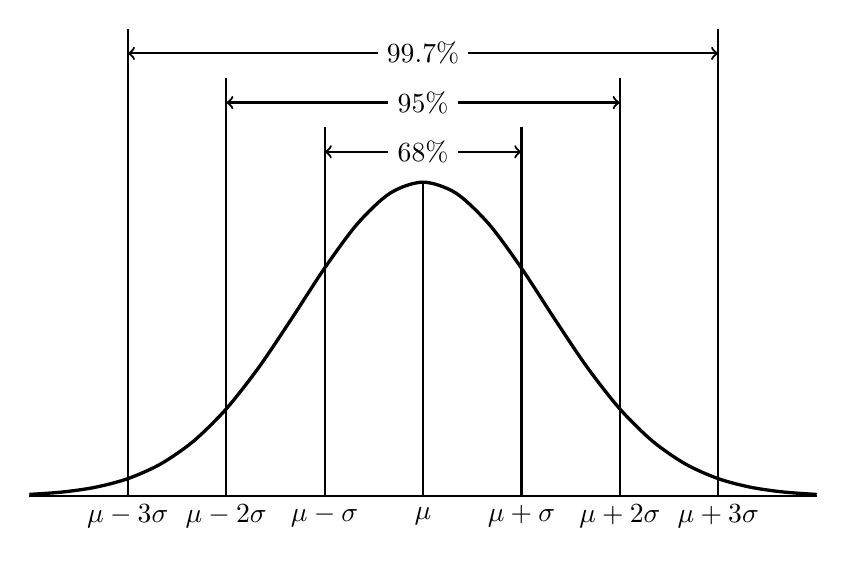
\begin{tikzpicture}[thick, domain=-4:4, scale=1.25]
	% axes
	\draw (-4, 0) -- (4, 0);
	\draw (+0, 0) -- (0, 3.18);
	\node at (-3, -0.2) {$\mu-3\sigma$};
	\node at (-2, -0.2) {$\mu-2\sigma$};
	\node at (-1, -0.2) {$\mu-\sigma$};
	\node at (+0, -0.2) {$\mu$};
	\node at (+1, -0.2) {$\mu+\sigma$};
	\node at (+2, -0.2) {$\mu+2\sigma$};
	\node at (+3, -0.2) {$\mu+3\sigma$};

	% gause function
	\def\gaussian#1#2{
		\draw[very thick, smooth] plot (\x, {10/(#2*sqrt(2*pi))*exp(-(\x-#1)^2/(2*#2^2))});
	}
	\gaussian{0}{1.25}

	% \percentage#std#y#percent
	\def\percentage#1#2#3{
		\draw (-#1, 0) -- (-#1, #2);
		\draw (+#1, 0) -- (+#1, #2);
		\draw[<->] (-#1, #2 - .25) -- (+#1, #2 - .25);
		\node[fill=white] at (0, #2 - .25) {#3\%};
	}
	\percentage{1}{3.75}{68}
	\percentage{2}{4.25}{95}
	\percentage{3}{4.75}{99.7}
\end{tikzpicture}
			\caption*{\textcolor{blue}{\textbf{Hình A.1:}} Tỷ lệ diện tích phân phối Gauss theo độ lệch chuẩn.}
		\end{figure}
	\end{frame}
	
	\begin{frame}[noframenumbering]
        \begin{block}{Thông tin mạch máu gan*}
			\begin{itemize}
				\item \textbf{Tĩnh mạch cửa} là mạch máu có đường kính lớn nhất trong cơ quan gan.
				\item Đường kính tĩnh mạch cửa trong khoảng \textbf{15 -- 18mm}.
			\end{itemize}
		\end{block}
	    \vspace{-10mm}\let\thefootnote\relax\footnote{\hspace{-3mm}\tiny *Nguồn:~A. M. Covey, L. A. Brody, G. I. Getrajdman, C. T. Sofocleous, and K. T. Brown, ``Incidence, patterns, and clinical relevance of variant portal vein anatomy,'' American Journal of Roentgenology, vol. 183, no. 4, pp. 1055–1064, 2004.}
    \end{frame}
\end{document}
